%!TEX TS-program = xelatex
%!TEX encoding = UTF-8 Unicode

% Load Thesis Class
\documentclass{DEIThesis}

\title{A Preliminary Study on Vowel Recognition using Convolutional Neural Networks for Individuals with Speech Disorders in the Italian Language}

\author{Huimin Chen}
\studentId{2071518}

% Advisor
\advisor{Prof. CANAZZA TARGON, SERGIO}

% % If you are co-advised
% \coadvisor{Dott. Robert Kahn}
% \coadvisorsUniversity{University of Princeton}

\university{University of Padova}
\mastername{Computer Engineering}
\academicYear{2024/2025}

\begin{filecontents*}[overwrite]{\jobname.xmpdata}
    \Title{A Preliminary Study on Vowel Recognition using Convolutional Neural Networks for Individuals with Speech Disorders in the Italian Language}
    \Author{Luca Martinelli}
    \Language{en-EN}
    \Keywords{Computer Engineering\sep LaTeX}
\end{filecontents*}

% Document

\begin{document}
    % The front matter (Cover, ToC, Abstract, etc...)
    \frontmatter

    % The main content
    \mainmatter
    
    %!TEX root = ../main.tex

\chapter{Introduction}
\label{chp:intro}

\paragraph{}
This thesis investigates the application of Convolutional Neural Networks (CNNs) in vowel recognition for Italian speech therapy, with a particular focus on supporting individuals with speech disorders. The research addresses the critical need for accessible and effective speech therapy tools, especially for children with hearing impairments. Through the development and implementation of an AI-based vowel recognition system, this work aims to enhance traditional speech therapy methods with modern technological solutions. The introduction chapter presents the research background, examines the challenges faced by deaf children, explores current speech training and rehabilitation approaches, and discusses the integration of artificial intelligence in speech therapy. This foundation sets the context for the technical developments and experimental results presented in subsequent chapters.


\section{Research Background}
\label{sec:background}

Speech disorders are a significant global health concern affecting millions of people worldwide. According to the World Health Organization, approximately 5\% of children have speech development disorders \cite{who2021}, with this percentage increasing in developing countries. These disorders can significantly impact a child's educational, social, and emotional development, creating barriers to effective communication and social integration.

Recent advances in digital technology and artificial intelligence have opened new possibilities for addressing speech disorders \cite{speech_therapy2023}. These technological innovations offer potential solutions to traditional therapy limitations, particularly in accessibility and consistency of treatment. Neural network-based approaches, in particular, have shown promising results in speech recognition and analysis tasks \cite{neural_speech2022}, suggesting their potential application in speech therapy.

Among various speech disorders, those related to hearing impairment present unique challenges. Congenital hearing impairment, affecting approximately 1-3 in 1000 newborns \cite{hearing2022}, is one of the primary causes of delayed speech development. These children face substantial difficulties in developing language skills naturally because they cannot receive adequate auditory feedback, which is crucial for speech development.

The impact of speech disorders extends far beyond mere communication difficulties. Research has demonstrated that children with speech disorders often experience reduced academic performance due to difficulties in classroom participation and comprehension. These challenges frequently lead to social isolation as children struggle to form relationships with their peers. The resulting social barriers can significantly affect their self-esteem and confidence, potentially leading to increased risk of mental health issues. Furthermore, these early challenges can have long-lasting effects, potentially limiting career opportunities and social advancement in later life.



\section{The Reality of Deaf Children}
\label{sec:deaf_children}

\begin{displayquote}
    "The greatest disability in society is not the physical limitation of people with disabilities, but rather the constructed limitation of people's thoughts about those disabilities."
    \\ -- Helen Keller
\end{displayquote}


Deaf children face unique and complex challenges in their developmental journey that extend far beyond the mere inability to hear. Current statistics reveal a concerning reality: approximately 90\% of deaf children are born to hearing parents \cite{deaf2023}, creating immediate and significant communication barriers within the family environment. This communication gap often leads to delayed language acquisition and emotional development, as parents struggle to establish effective early communication methods with their children \cite{family_support2022}.

The educational landscape for deaf children presents additional challenges. Research indicates that deaf children in mainstream educational settings often experience significant academic difficulties, with many falling behind their hearing peers in various subjects \cite{deaf_education2023}. This academic gap is not due to any inherent cognitive differences but rather stems from communication barriers and inadequate educational support systems. More troubling is the fact that only 30\% of deaf children receive early intervention services, despite overwhelming evidence supporting the critical importance of early support for language development and cognitive growth.

\paragraph{}
Social integration represents another significant challenge for deaf children. Studies have shown that deaf children often experience social isolation and difficulties in peer relationships, which can have long-lasting effects on their emotional well-being and self-esteem \cite{social_integration2023}. The challenge of navigating between the deaf and hearing worlds can create a sense of cultural displacement, as children struggle to establish their identity and find their place in both communities.

\paragraph{}
Early intervention programs have emerged as a crucial factor in supporting deaf children's development. Research demonstrates that children who receive appropriate early intervention services show significantly better outcomes in language development, cognitive skills, and social adjustment \cite{early_intervention2022}. However, access to these services remains limited, with less than half of deaf children having regular access to speech therapy and other essential support services.

\paragraph{}
The role of technology in supporting deaf children's development has become increasingly significant. Modern assistive technologies and digital communication tools have opened new possibilities for learning and interaction \cite{technology_impact2023}. However, the digital divide and economic disparities mean that many children, particularly in underserved communities, lack access to these potentially transformative resources.

\paragraph{}
The family environment plays a crucial role in a deaf child's development. Parents of deaf children often face significant challenges in adapting their communication methods and learning new skills to support their child's development. Studies show that families who receive proper support and training in communication strategies are better equipped to foster their child's language development and emotional well-being \cite{family_support2022}. However, many families lack access to these support systems, creating additional barriers to their child's development.

\paragraph{}
The intersection of deafness with other aspects of identity and social circumstances adds another layer of complexity. Factors such as socioeconomic status, cultural background, and geographical location can significantly impact a deaf child's access to resources and opportunities for development. This intersectionality requires careful consideration in developing support systems and interventions that can effectively address the diverse needs of deaf children and their families.

\section{Speech Training and Rehabilitation}
\label{sec:speech_training}

\paragraph{}
Speech rehabilitation training plays a crucial role in the language development of children with hearing impairments. Research consistently shows that early intervention and systematic speech training can significantly improve children's language abilities \cite{early2021}. The critical period for language development occurs during the first few years of life, making early intervention essential.

\paragraph{}
Modern speech rehabilitation encompasses a diverse range of methodologies and approaches \cite{speech_methods2023}. Traditional face-to-face therapy sessions remain fundamental but are increasingly complemented by innovative digital solutions. These methods include articulation therapy, phonological process approaches, and motor-based interventions. Each approach is tailored to address specific aspects of speech development, from basic sound production to complex language patterns.

\paragraph{}
The integration of digital platforms has revolutionized speech therapy practices \cite{digital_therapy2022}. These technological advances have introduced several transformative capabilities to the field. Real-time feedback mechanisms now allow learners to visualize their speech patterns with unprecedented clarity. Gamified exercises have proven effective in maintaining engagement and motivation throughout the therapy process. Advanced progress tracking tools enable therapists to make data-driven adjustments to treatment plans. Remote therapy options have significantly increased accessibility for many patients. Furthermore, automated practice sessions effectively supplement traditional therapy approaches, providing consistent support between formal sessions.

\paragraph{}
Motivation has emerged as a critical factor in the success of speech rehabilitation programs, particularly for young learners. Recent studies have identified several key elements that significantly influence engagement and persistence in therapy \cite{motivation_speech2023}. Interactive and age-appropriate activities form the foundation of successful engagement strategies. Clear visualization of progress helps maintain motivation by making improvements tangible and measurable. Positive reinforcement systems have proven essential in encouraging continued effort. Strong social support networks provide emotional backing and encouragement. Achievement recognition mechanisms help celebrate progress and maintain long-term commitment to the rehabilitation process.

\paragraph{}
The emergence of telerehabilitation has significantly transformed speech therapy delivery \cite{telerehab2022}. This innovative approach has brought numerous benefits to the field, particularly in terms of accessibility for remote communities. Reduced travel time and costs have made therapy more feasible for many families. Flexible scheduling options have allowed more consistent participation in therapy sessions. However, this approach also presents unique challenges. Technology barriers can impede effective delivery of services, connectivity issues may disrupt sessions, and some therapeutic techniques require modification to suit the online environment.

\paragraph{}
Traditional speech therapy methods continue to play a vital role in rehabilitation. One-on-one sessions with speech therapists provide personalized attention and immediate feedback. Group therapy sessions offer opportunities for peer learning and social interaction. Home-based exercises reinforce learning and promote consistent practice. Visual feedback systems and parent-mediated interventions complement these traditional approaches, though each method brings its own advantages and limitations.

\paragraph{}
Contemporary rehabilitation programs increasingly adopt multimodal approaches \cite{multimodal2023}. Traditional articulation exercises form the foundation of these programs, supplemented by sophisticated visual feedback systems. Tactile cues and physical prompts help learners develop proper articulation patterns. Rhythm and music-based activities enhance engagement and facilitate natural speech patterns. Augmentative and alternative communication tools provide additional support when needed, creating a comprehensive therapeutic environment.

\paragraph{}
The Italian language presents unique challenges and opportunities in speech therapy. Its relatively regular vowel system makes it an ideal candidate for systematic speech training \cite{italian_phonetics2021}. The clear distinction between Italian vowels provides a structured framework for developing and evaluating speech recognition systems, while also offering clear targets for learners to achieve.

\paragraph{}
Current speech training approaches face significant challenges in practice. The availability of qualified therapists is often limited, particularly in rural or underserved areas. The high cost of regular therapy sessions creates financial barriers for many families. Geographic distance to therapy centers can make regular attendance difficult or impossible for some families. Additionally, maintaining consistent child engagement between sessions proves challenging, and the practice between sessions often lacks the consistency needed for optimal progress.

\paragraph{}
The future of speech rehabilitation lies in the integration of traditional therapeutic approaches with emerging technologies. This combination promises to address many current limitations while maintaining the essential human element of therapy. Success in this field requires careful consideration of individual needs, technological capabilities, and evidence-based practices to ensure optimal outcomes for each learner.

\section{AI Integration in Speech Training}
\label{sec:ai_integration}

\paragraph{}
Artificial Intelligence offers promising solutions to enhance traditional speech therapy methods. Through personalized learning approaches, AI systems can adapt difficulty levels to individual needs, track progress comprehensively, and provide customized feedback that evolves with the child's development. This personalization ensures that each child receives training tailored to their specific needs and learning pace.

\paragraph{}
The continuous availability of AI-based systems represents a significant advantage. Unlike traditional therapy sessions, these tools can be accessed 24/7, providing consistent feedback and enabling remote learning capabilities. This accessibility helps maintain regular practice schedules and ensures that learning can continue beyond the confines of scheduled therapy sessions.

\paragraph{}
Enhanced engagement through AI systems comes through carefully designed interactive exercises and real-time visual feedback. By incorporating gamification elements, these systems can maintain children's interest and motivation, making the learning process more enjoyable and effective. The immediate feedback helps children understand their progress and encourages continued practice.

\paragraph{}
The integration of gamification elements in speech therapy applications has shown particular promise in maintaining children's engagement \cite{child_engagement2023}. These approaches transform traditional exercises into interactive experiences, making practice more enjoyable and sustainable. The combination of AI-driven feedback with game-like elements creates an environment where children are motivated to practice consistently, leading to better outcomes.

\subsection{Focus on Vowel Training}
\label{subsec:vowel_focus}

\paragraph{}
The effectiveness of AI-based speech therapy systems has been demonstrated in several studies \cite{ai_speech2022}. These systems have shown particular success in providing consistent, objective feedback that complements traditional therapy approaches. The ability to collect and analyze detailed data about a child's progress allows for more precise tracking of development and enables therapists to make more informed decisions about treatment strategies.

\paragraph{}
In speech training, vowel recognition and production serve as fundamental building blocks. Vowels represent the basic units of language and significantly impact overall speech intelligibility \cite{vowel2020}. They provide an essential foundation for developing more complex speech sounds, and their relatively consistent acoustic patterns make them ideal candidates for initial speech training efforts. The focus on vowel training allows for clear measurement of progress and provides immediate feedback that can motivate continued learning.

\paragraph{}
The primacy of vowels in speech development is well-established through extensive research \cite{speech_methods2023}. Vowels carry approximately more than half of the speech signal's energy and form the core of syllabic structure in most languages. Their proper articulation is crucial for word recognition and overall communication effectiveness. For children with hearing impairments, mastering vowel production becomes particularly critical as these sounds provide the foundation for developing proper prosody and intonation patterns.

\paragraph{}
From a developmental perspective, vowel training offers several strategic advantages. First, vowels are typically produced with relatively stable articulatory configurations, making them easier to teach and learn compared to consonants. Second, vowels are sustained sounds that can be held and modified, allowing learners to receive extended feedback and make real-time adjustments. Third, the acoustic properties of vowels are more distinct and consistent than those of consonants, facilitating both automated recognition and human perception \cite{multimodal2023}.

\paragraph{}
The choice to focus on vowel recognition in Italian is supported by both linguistic and practical considerations. Italian vowels are particularly well-suited for computer-based recognition due to their distinct acoustic properties \cite{italian_phonetics2021}. The Italian vowel system, with its seven phonemic vowels, provides a clear and systematic framework for training. Each vowel occupies a distinct position in the acoustic space, making it easier for learners to perceive and reproduce the differences between sounds. This characteristic makes them ideal candidates for developing and testing AI-based recognition systems, while also providing clear benchmarks for measuring improvement in speech production.

\paragraph{}
The systematic nature of vowel training also facilitates the development of structured learning programs. By focusing initially on vowels, therapists can establish clear progression paths, moving from simple sustained vowels to more complex combinations in different phonetic contexts. This structured approach allows for better monitoring of progress and more effective adaptation of training strategies. Furthermore, success in vowel production often leads to increased confidence and motivation, encouraging learners to tackle more challenging aspects of speech production \cite{motivation_speech2023}.

\paragraph{}
In the context of digital speech therapy, vowel training presents unique opportunities for technological innovation. The relatively simple acoustic patterns of vowels make them ideal for real-time analysis and feedback systems. Advanced visualization techniques can represent vowel production in ways that are both accurate and intuitive for learners. This combination of clear acoustic targets and immediate visual feedback creates an effective learning environment, particularly beneficial for children who rely heavily on visual cues due to hearing impairments \cite{digital_therapy2022}.

\paragraph{}
Moreover, the focus on vowel training aligns well with the needs of both learners and therapists. For learners, particularly children, the ability to produce clear, distinct vowels provides an immediate sense of achievement and progress. For therapists, the systematic nature of vowel training offers clear metrics for assessment and progress tracking. This alignment of pedagogical needs with technological capabilities makes vowel training an ideal starting point for implementing AI-assisted speech therapy solutions.

\section{Thesis Structure}
\label{sec:structure}

\paragraph{}
This thesis is organized into eight chapters that systematically present our research on vowel recognition using CNNs:

\paragraph{}
Chapter 1 (Introduction) presents the research background, examining the challenges faced by deaf children and exploring current speech training approaches. It introduces the motivation for developing AI-based solutions for speech therapy and establishes the context for our work.

\paragraph{}
Chapter 2 (State of the Art) provides a comprehensive review of current speech recognition technology, with particular focus on vowel recognition systems and their applications in the Italian language. It traces the evolution from traditional methods to modern deep learning approaches.

\paragraph{}
Chapter 3 (SoundRise: the Background Idea) introduces the SoundRise application, detailing its historical development and evolution. This chapter explains the fundamental concept and overall functionality of the application, particularly focusing on its role in speech therapy.

\paragraph{}
Chapter 4 (CNN in Classification) presents a detailed examination of Convolutional Neural Networks and their application in image classification tasks. It covers the theoretical foundations and architectural components that make CNNs particularly suitable for spectrogram-based vowel recognition.

\paragraph{}
Chapter 5 (CNN Vowel Recognition Model) describes our implementation of the CNN model for vowel recognition. It details the audio data preparation pipeline, spectrogram generation process, and the specific CNN architecture developed for this application.

\paragraph{}
Chapter 6 (Experimental Results and Analysis) presents comprehensive experimental results, including model performance across different configurations, classification accuracy for each vowel, and detailed analysis of the system's effectiveness.

\paragraph{}
Chapter 7 (Web Application Implementation) details the technical implementation of the SoundRise web application, including system architecture, frontend and backend components, deployment process, and user interface design. It also provides complete instructions for setting up and testing the application.

\paragraph{}
Chapter 8 (Conclusions and Future Works) summarizes the key achievements of this research, discusses its implications for speech therapy applications, and outlines potential directions for future work, including data collection strategies and technical enhancements.

\paragraph{}
The thesis concludes with a comprehensive bibliography and any necessary appendices containing additional technical details and supplementary materials.


    %!TEX root = ../main.tex

\chapter{State of the Art}
\label{chp:stateOfArt}

\paragraph{}
This chapter provides a comprehensive review of the current state of speech recognition technology, with a particular focus on vowel recognition systems and their applications in the Italian language. The chapter begins by tracing the evolution of speech recognition technology from its early beginnings to modern deep learning approaches. Special attention is given to the development of vowel recognition systems, examining both traditional acoustic-phonetic methods and contemporary neural network-based solutions. The unique characteristics of the Italian vowel system and its implications for speech recognition are thoroughly explored. Additionally, the chapter discusses current applications in speech therapy, technical challenges, and future research directions, providing a foundation for understanding the context and significance of this research.

\section{Evolution of Speech Recognition Technology}
\label{sec:evolution}

\paragraph{}
Speech recognition technology has undergone a remarkable transformation over the past several decades, with particularly significant advances in vowel recognition systems \cite{deep_speech2023}. This evolution reflects the broader progression of artificial intelligence and machine learning technologies, but with specific applications in speech therapy and language learning. The journey from basic pattern matching to sophisticated neural networks represents not just technological advancement, but a fundamental shift in how we approach speech recognition and rehabilitation. Early systems in the 1950s and 1960s could only recognize isolated phonemes with limited accuracy, while modern systems can process continuous speech in real-time with remarkable precision \cite{acoustic_analysis2023}.

\paragraph{}
The historical development of speech recognition can be traced through several distinct phases. The initial phase, spanning the 1950s to 1970s, focused on acoustic-phonetic approaches, attempting to identify distinct units of sound based on their acoustic properties. This was followed by the pattern-recognition approach in the 1970s and 1980s, which introduced statistical methods and template matching. The 1980s and 1990s saw the rise of hidden Markov models (HMMs) and statistical learning methods, which dominated the field for several decades \cite{formant_analysis2022}. Each of these phases contributed essential insights and methodologies that continue to influence modern approaches.

\paragraph{}
The transition to modern deep learning approaches began in the early 2010s, marking a revolutionary change in speech recognition capabilities \cite{cnn_vowels2023}. This shift was enabled by several key developments: the availability of large-scale speech datasets, significant increases in computing power, and breakthroughs in neural network architectures. Deep learning models, particularly Convolutional Neural Networks (CNNs) and Recurrent Neural Networks (RNNs), demonstrated unprecedented accuracy in speech recognition tasks. These advances were especially significant for vowel recognition, as the complex spectral patterns that distinguish vowels could be learned automatically from data, rather than requiring hand-crafted features.

\paragraph{}
In the specific context of speech therapy and rehabilitation, this technological evolution has enabled increasingly sophisticated applications. Early computer-aided speech therapy systems were limited to basic visualization of acoustic parameters, such as pitch and intensity. Modern systems, however, can provide detailed, real-time feedback on multiple aspects of speech production, including precise vowel articulation, prosody, and voice quality \cite{italian_therapy2023}. The integration of machine learning has made these systems more adaptive and personalized, capable of adjusting to individual user needs and learning patterns.

\paragraph{}
Recent developments have focused on creating more robust and versatile recognition systems that can handle variations in speech patterns, accents, and environmental conditions. This is particularly crucial for applications in speech therapy, where users may have non-standard pronunciation patterns or speech disorders. Advanced neural network architectures, combined with sophisticated signal processing techniques, have made it possible to achieve high recognition accuracy even in challenging conditions \cite{adaptive_learning2023}. These improvements have been especially beneficial for vowel recognition systems, which require precise discrimination between similar sounds.

\paragraph{}
The current state of speech recognition technology represents a convergence of multiple approaches, combining the best aspects of traditional signal processing with modern machine learning methods. This hybrid approach has proven particularly effective for specialized applications such as vowel recognition in speech therapy. The ability to process and analyze speech in real-time, provide immediate feedback, and adapt to individual users has opened new possibilities for speech therapy and language learning applications.

\section{Vowel Recognition Systems}
\label{sec:vowel_recognition}

\subsection{Traditional Approaches}
\label{subsec:traditional}

\paragraph{}
Traditional vowel recognition systems primarily relied on acoustic feature extraction and formant analysis \cite{acoustic_analysis2023}. These methods focused on identifying and tracking formant frequencies, which are particularly crucial for vowel identification. The first two formants (F1 and F2) typically provide sufficient information for distinguishing between different vowels, making them fundamental parameters in vowel recognition systems.

\paragraph{}
Formant tracking techniques, including Linear Predictive Coding (LPC) and spectral analysis, formed the backbone of early vowel recognition systems. These approaches were particularly effective for controlled environments but faced challenges with speaker variability and background noise. The relationship between formant frequencies and vowel identity has been well-established through extensive research, providing a solid foundation for automated recognition systems.

\subsection{Modern Deep Learning Methods}
\label{subsec:deeplearning}

\paragraph{}
Recent advances in deep learning have transformed vowel recognition capabilities \cite{cnn_speech2022}. Convolutional Neural Networks (CNNs) have proven particularly effective in analyzing spectrograms of vowel sounds, offering superior feature learning capabilities and improved robustness to variations in pronunciation. These networks excel at capturing the subtle spectral patterns that distinguish different vowels.

\paragraph{}
Modern architectures incorporate adaptive learning mechanisms that can adjust to individual speaker characteristics \cite{adaptive_learning2023}. This adaptability is especially valuable in speech therapy applications, where the system must accommodate various pronunciation patterns and degrees of speech impairment. The ability to learn from individual speech patterns has significantly improved recognition accuracy for non-standard pronunciations.

\section{Italian Vowel Recognition}
\label{sec:italian_vowels}

\paragraph{}
The Italian vowel system is characterized by seven distinct phonemic vowels: /i/, /e/, /open-e/, /a/, /open-o/, /o/, and /u/. Each vowel occupies a unique position in the acoustic space, which is advantageous for both recognition systems and language learners. The clear separation of these vowel sounds facilitates accurate identification and pronunciation.

\paragraph{}
Recent research in Italian vowel recognition has focused on applying deep learning techniques to address the specific challenges of the Italian phonetic system. The relatively regular structure of Italian vowels, combined with their distinct acoustic properties, makes them an ideal target for machine learning approaches. Studies have shown that Convolutional Neural Networks (CNNs) are particularly effective at capturing the subtle spectral differences between similar vowel pairs, such as /e/ and /open-e/, as well as /o/ and /open-o/, which are crucial distinctions in Italian pronunciation.

\paragraph{}
The acoustic characteristics of Italian vowels have been extensively studied through formant analysis \cite{formant_analysis2022}. The first two formants (F1 and F2) show consistent patterns that distinguish between different vowels, creating well-defined acoustic targets for recognition systems. This regularity has facilitated the development of both traditional and neural network-based recognition approaches. Modern systems leverage these acoustic properties while adding the capability to handle natural variations in pronunciation and speaker characteristics.

\paragraph{}
Clinical applications of Italian vowel recognition systems have demonstrated particular promise in speech therapy settings \cite{italian_therapy2023}. These systems provide real-time feedback on vowel production accuracy, helping users visualize and correct their pronunciation. The integration of machine learning techniques has improved the systems' ability to handle non-standard pronunciations, making them especially valuable for working with speech disorders. Recent studies have shown significant improvements in pronunciation accuracy when using these computer-aided systems, particularly for children with hearing impairments.

\paragraph{}
The development of mobile and web-based applications for Italian vowel recognition has expanded access to these tools \cite{mobile_speech2022}. These platforms typically combine acoustic analysis with interactive interfaces, making practice more engaging and effective. The ability to practice independently, with immediate feedback, has proven particularly valuable for maintaining consistent progress between therapy sessions. Modern applications often incorporate adaptive learning mechanisms that can adjust to individual speech patterns while maintaining the standard targets of Italian vowel pronunciation.

\section{Speech Therapy Applications}
\label{sec:applications}

\subsection{Computer-Aided Vowel Training}
\label{subsec:computer-aided}

\paragraph{}
Modern computer-aided speech training systems specifically designed for Italian vowel recognition employ various innovative approaches \cite{italian_therapy2023}. Real-time visualization of vowel production provides immediate feedback on articulation accuracy. These systems typically integrate acoustic analysis with visual feedback, helping users understand and correct their pronunciation patterns. Mobile applications have made these tools more accessible \cite{mobile_speech2022}, enabling consistent practice outside traditional therapy settings.

\paragraph{}
Gamification elements have proven particularly effective in vowel training applications \cite{gamification2023}. Interactive exercises focused on specific vowel contrasts help maintain engagement while providing structured practice opportunities. The immediate feedback on vowel production accuracy helps learners develop better awareness of their articulation patterns.

\section{Technical Challenges}
\label{sec:challenges}

\paragraph{}
Vowel recognition systems face several specific challenges in the context of speech therapy. Real-time processing requirements demand efficient algorithms that can provide immediate feedback while maintaining accuracy. Environmental noise and microphone quality can significantly impact formant detection accuracy. Speaker variability, particularly in the case of speech disorders, requires robust recognition models that can handle non-standard pronunciations.

\paragraph{}
The development of Italian-specific vowel recognition systems involves additional considerations. Distinguishing between similar vowel pairs, such as /e/ and its open variant, as well as /o/ and its open variant, requires high-precision acoustic analysis. These systems must also account for regional variations in Italian vowel pronunciation while maintaining consistent recognition standards.

\section{Summary}
\label{sec:summary}

\vspace{0.5cm}

\paragraph{}
This chapter has reviewed the current state of research in speech therapy, focusing on the evolution of speech recognition technology and its applications in vowel recognition systems, particularly within the Italian language. It has explored both traditional and modern deep learning approaches, highlighting the advancements in neural network architectures that have significantly improved recognition accuracy. The chapter also discussed the unique characteristics of the Italian vowel system and its implications for speech therapy applications, addressing technical challenges and future research directions. Overall, this comprehensive review provides a foundation for understanding the context and significance of ongoing research in this field.


    %!TEX root = ../main.tex

\chapter{SoundRise: the Background Idea}
\label{chp:background}

\paragraph{}
This chapter explains the fundamental concept and overall functionality of the SoundRise application, detailing its past versions. Specifically, a focus will be placed on its reactivation based on models studied and defined inside the CSC (Centro di Sonologia Computazionale), and the procedural aspects of applying reactivation to SoundRise will be delineated.

\section{What is SoundRise}
\label{sec:what-is-soundrise}

\paragraph{}
SoundRise is an innovative educational game designed to support children in discovering and understanding their vocal abilities. It serves as a complementary tool to traditional speech therapy, offering an engaging and interactive platform for autonomous learning. The application is particularly beneficial for children with hearing impairments, providing them with a unique opportunity to explore their vocal capabilities in a supportive environment.

\paragraph{}
The core aim of SoundRise, since its inception about 10 years ago, has been to create an interactive application that utilizes real-time analysis of vocal features. This approach helps children understand how their voice works by providing immediate visual feedback. The application employs advanced audio processing techniques to analyze vocal input, allowing users to see a graphical representation of their voice in real-time.

\paragraph{}
SoundRise is particularly focused on helping deaf children acquire a deep understanding of their vocal capabilities. The application uses a playful metaphor of a sleeping sun that reacts to the child's voice. When the sun hears a sound, it opens its eyes and changes its appearance and position. This visual feedback is crucial for children to monitor their progress and make necessary adjustments to their vocal output.

\paragraph{}
The sun's movements are directly linked to the vocal input: it rises and falls vertically according to the pitch of the sound emitted, grows bigger or smaller depending on the sound intensity, and changes color based on the vocal timbre detected. This color change is associated with the identification of the five vowels of the Italian language, with each vowel corresponding to a different color of the sun. This innovative approach not only makes learning fun but also enhances the child's ability to recognize and produce different vowel sounds.



\paragraph{}
In Figure 3.1, the first interface of the SoundRise application, developed by Stefano Giusto \cite{giusto2012} in Pure Data, is shown. This interface, running on a PC in the CSC, laid the foundation for subsequent developments and improvements in the application, as detailed in the following sections.


\paragraph{}
The child's voice is interpreted by a sleeping sun. When the sun hears a sound (i.e. when the microphone recognises a sound), it opens its eyes and changes its appearance and position. The change of the sun depends on the changing sound expressed by the child's voice. The sun can rise and fall vertically according to the pitch of the sound emitted. It can grow bigger or smaller depending on the sound intensity. The sun also changes its colour, based on the vocal timbre detected. The recognition of this property is related to the identification of the five vowels of the Italian language: graphically, each possible timbre (5, as the vowels) corresponds to a different colour of the sun.

\paragraph{}
By providing a visual representation of the emitted sound, SoundRise helps children correct their pronunciation and improve their vocal skills. The application is designed to be intuitive and user-friendly, ensuring that even young users can navigate it with ease. The engaging interface and immediate feedback make it an effective tool for speech therapy, encouraging children to practice and improve their vocal abilities.

\paragraph{}
Therefore, the application uses the user's vocal input to create an interactive visual experience, providing to the child a visual feedback on the emitted sound of his/her voice, helping him/her to correct himself/herself, with the aim of educating him/her in the use of his/her own voice.

\paragraph{}
In Figure 3.1 it is possible to see the first interface of the SoundRise application, developed by Stefano Giusto \cite{giusto2012} in Pure Data (more details in the next sections) that is running on a PC in the CSC.

\begin{figure}[h]
    \centering
    \includegraphics[width=0.8\textwidth]{res/images/background/soundrise-1.png}
    \caption{First interface of the SoundRise application}
    \label{fig:soundrise-logo}
\end{figure}

\section{The Evolution of SoundRise Over Time}
\label{sec:evolutionOfSoundRise}

\paragraph{}
The first idea for SoundRise was sketched out by Prof. Federico Avanzini, Prof. Antonio Rodà and Prof. Sergio Canazza from the Department of Information Engineering at the University of Padua, in collaboration with Dr. Serena Zanolla from the University of Udine. From then on, the project started to develop in the CSC (Centro di Sonologia Computazionale) at the University of Padua.

\paragraph{}
The initial development of SoundRise was carried out through three significant master thesis projects at the University of Padua. In 2012, two foundational theses were completed: Stefano Giusto's work (Giusto S. Rodà A., SoundRise: Studio e Progettazione Di un'Applicazione Multimodale Interattiva Per La Didattica Basata sull'Analisi Di Feature Vocali) \cite{giusto2012} and Marco Randon's research (Randon M. Avanzini F., SoundRise: Sviluppo E Validazione Di un'Applicazione Multimodale Interattiva Per La Didattica Basata Sull'analisi Di Feature Vocali) \cite{randon2012}. More recently, in 2023, Giada Zuccolo's thesis "A New Sunrise for Speech Therapy: Development of SoundRise 2.0 Application" \cite{zuccolo2023} brought significant advancements to the project, focusing on modernizing the application and enhancing its therapeutic capabilities.

\paragraph{}
These three master theses collectively established and evolved SoundRise as a comprehensive educational-therapeutic tool. The initial versions developed by Giusto and Randon laid the foundation as a standalone application aimed at supporting vocal therapy and voice modulation practice for young users. Zuccolo's recent contribution further enhanced the system by implementing new features and improving the user experience for both therapists and children.

\paragraph{}
In the master thesis of Stefano Giusto \cite{giusto2012}, the application was developed using the real-time graphical programming environment Pure Data\footnote{Pure Data (Pd) is an open source visual programming language for multimedia.} \cite{puredata2015} and the external library timbreID for vocal timbre analysis. timbreID \cite{timbreid2016} represents a collection of externals for Pd, developed by William Brent. The features generated through the external objects can be used directly as control information in real-time performance. This library consists of a group of objects for extracting timbre features and a classification object that manages the resulting database of information. The incoming audio signal is processed by a specific object that detects attacks, defined as abrupt changes in the spectral envelope of the incoming sound, and generates a maximum match relation.

\paragraph{}
Subsequently, in the master thesis of Marco Randon \cite{randon2012}, the application was modified to enhance its portability across different platforms. To achieve this, it became necessary to modify its architecture in a manner that would allow it to run independently of Pd while maintaining its core features and functionalities. Moreover, efforts were made to improve its graphical interface to adapt it for touchscreen devices. This new version of the application was developed in C++ language and using the libpd library for the communication with Pd. In essence, libpd consists of variations of processing callback functions for different sample types, a set of functions for sending messages to Pd, and a series of function pointers for receiving messages from Pd. In order to receive messages, the client code must implement the appropriate receive functions and assign them to the corresponding function pointers in libpd.

\paragraph{}
libpd includes language wrappers (C++, and others) that make libpd's functionality available to the respective programming language. These wrappers perform data type conversions between Pd's custom data types and the standard data types of the target language. They provide an object-oriented interface for message exchange functions and function pointers. To receive messages from Pd, the client code must implement the necessary methods of the PdReceiver interface and register a receiver object using the methods of the PdBase class.

\paragraph{}
A more detailed study of the functioning of SoundRise was carried out by Riccardo Fila (Canazza Targon S., Fiordelmondo A., Fila R., SoundRise 2.0: Sviluppo di un modello di riconoscimento timbrico per un sistema di assistenza web dedicato a persone con disabilità uditive) \cite{fila2020}. In this thesis, that is the last project related with SoundRise before this thesis, an in-depth study was carried out in order to develop a timbre recognition model. This project was developed in Javascript with the aid of Web Audio API (explained in detail in the chapter 4, on the section 4.2). Basically, a function calculates the first two formant frequencies of the voice and compares them with those characteristic of Italian vowels in order to find an effective match and display it graphically. The idea of developing this type of application on the web was a turning point, as will be explained in Chapters 4 and 5, mainly because of the possibility of being able to exploit the potential of the Web Audio API.

\paragraph{}
In Figure 3.2, it is possible to see the interface of this prototype, so how it works: after starting the microphone, it analyses voice data and shows the resulting vowel (when it is able to capture it): the yellow column shows the vowel that was recognised by the model (if it was recognised), while the subsequent green columns show the analysed frequency values.

\begin{figure}[h]
    \centering
    \includegraphics[width=0.8\textwidth]{res/images/soundrise-1.png}
    \caption{SoundRise web prototype interface}
    \label{fig:soundrise-1}
\end{figure}



\paragraph{}
The formant frequencies play a crucial role in vowel recognition within the Italian language system. Each vowel has its distinct characteristic formant frequencies that serve as acoustic signatures. For the vowel /a/, the first formant (F1) typically occurs around 800Hz, while the second formant (F2) is found near 1400Hz, creating its characteristic open sound. The vowel /e/ exhibits F1 at approximately 400Hz and F2 at 2000Hz, producing its mid-front quality. The high front vowel /i/ is characterized by a low F1 of about 250Hz and a high F2 of 2250Hz. The back vowel /o/ shows F1 around 400Hz and F2 near 800Hz, while /u/ has F1 at approximately 250Hz and F2 at 600Hz, creating its distinctive high back quality.

\paragraph{}
The duration of vowel sounds represents another critical parameter in speech analysis and recognition. In natural speech, Italian vowels typically range from 100 to 300 milliseconds in duration. This duration can vary significantly based on factors such as speaking rate, stress patterns, and phonetic context. In stressed positions, vowels tend toward the longer end of this range, while unstressed vowels are generally shorter. This temporal characteristic provides important cues for both speech recognition systems and human listeners.

\paragraph{}
Intensity patterns also serve as distinctive features for vowel identification. Each vowel exhibits characteristic amplitude patterns that contribute to its unique acoustic profile. These patterns are influenced by the specific configuration of the vocal tract during production and play a crucial role in vowel perception. High vowels like /i/ and /u/ typically show lower intrinsic intensity compared to low vowels like /a/, due to physiological factors in their production. Understanding these intensity patterns is essential for developing accurate vowel recognition systems.

\paragraph{}
These acoustic parameters - formant frequencies, duration, and intensity - form the foundation of vowel recognition in SoundRise. The application's analysis system carefully monitors these characteristics in real-time, enabling accurate identification of the produced vowels and providing appropriate visual feedback through the sun interface. This comprehensive approach to vowel analysis ensures reliable recognition across different speakers and speaking conditions.

\section{SoundRise 2.0: A New Era}
\label{sec:soundrise-2}

\paragraph{}
The most recent and significant evolution of SoundRise came through Giada Zuccolo's master thesis "A New Sunrise for Speech Therapy: Development of SoundRise 2.0 Application" \cite{zuccolo2023}, supervised by Professor Sergio Canazza Targon and co-supervised by Dott. Alessandro Fiordelmondo. This work represents a fundamental shift in the application's architecture and capabilities, establishing the foundation for modern speech therapy applications.

\paragraph{}
SoundRise 2.0 introduced a complete architectural overhaul, moving away from the traditional standalone application model to a modern web-based architecture. The application was rebuilt using React.js for the frontend, providing a responsive and intuitive user interface. The backend implementation utilized Python, enabling robust audio processing and analysis capabilities. This architectural decision significantly improved accessibility and maintainability while facilitating future enhancements.

\begin{figure}[h]
    \centering
    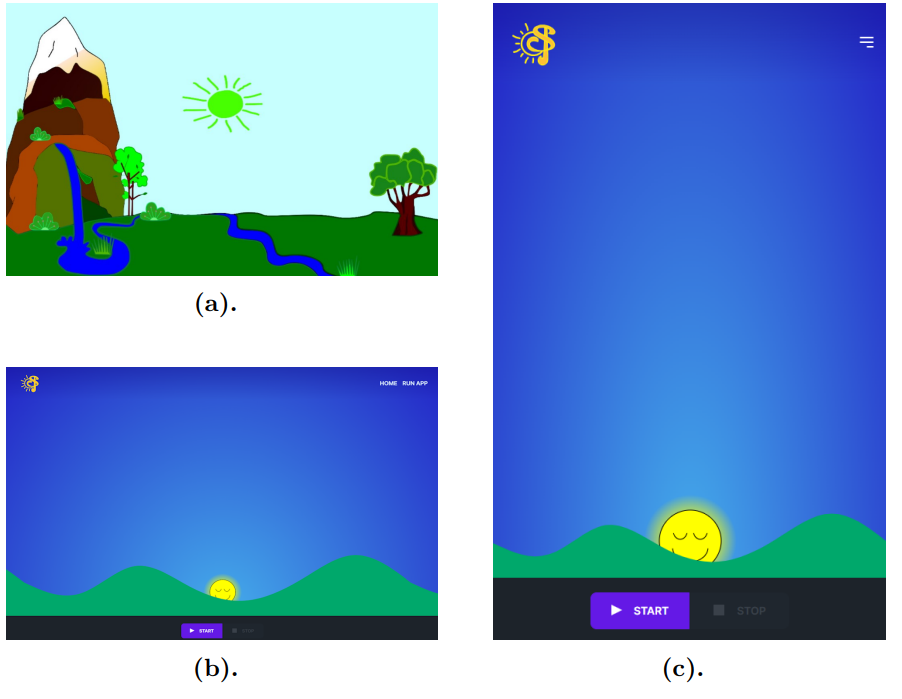
\includegraphics[width=0.8\textwidth]{res/images/background/soundrise-2.png}
    \caption{SoundRise web prototype interface}
    \label{fig:soundrise-2}
\end{figure}

\paragraph{}
The new version brought substantial improvements to the user interface, maintaining the engaging sun metaphor while introducing more sophisticated visual feedback mechanisms. The interface was designed with particular attention to the needs of young users and speech therapists. At its core, the application features intuitive controls for audio recording and playback, ensuring that even young users can easily navigate and interact with the system. The real-time visual feedback system provides immediate response to vowel pronunciation, helping users understand and correct their articulation patterns. Progress tracking has been enhanced with clear indicators and achievement metrics, allowing both users and therapists to monitor improvement over time. The responsive design ensures optimal functionality across various device sizes, making the application accessible in different therapeutic settings.


\paragraph{}
Zuccolo's implementation brought several significant technical improvements to the platform. The integration of the Web Audio API enables precise audio capture and analysis, providing the foundation for accurate vowel recognition. Advanced audio processing algorithms were implemented to enhance the quality and reliability of speech analysis. The addition of real-time spectrogram generation and analysis provides detailed insights into vowel pronunciation patterns. The formant analysis system was significantly improved, leading to more accurate vowel recognition across different speakers and acoustic conditions.


\paragraph{}
SoundRise 2.0 was developed with a strong focus on clinical applicability, incorporating features essential for therapeutic use. The application supports structured therapy sessions through a carefully designed progression of exercises and activities. A comprehensive progress tracking system allows therapists to monitor and document patient improvement over time. The platform enables customization of exercises based on individual patient needs and therapeutic goals. Additionally, the system facilitates effective communication between therapists and patients, creating a collaborative environment for speech therapy.


\paragraph{}
Zuccolo's work on SoundRise 2.0 has established a robust foundation for future developments in speech therapy applications. The modular architecture and modern technology stack enable continuous improvement and feature expansion. This version serves as the basis for subsequent research and development, including the current work on implementing CNN-based vowel recognition systems, which aims to further enhance the application's accuracy and effectiveness in speech therapy settings.

\paragraph{}
The success of SoundRise 2.0 in combining technical innovation with clinical utility has opened new possibilities for computer-aided speech therapy. The application demonstrates how modern web technologies and thoughtful design can create effective tools for speech therapy, particularly for children with hearing impairments. This foundation continues to evolve through ongoing research and development efforts at the University of Padua.

\section{Summary}
\label{sec:summary}

\vspace{0.5cm}

\paragraph{}
This chapter has provided an in-depth look at the SoundRise application, detailing its origins, core functionalities, and the innovative methodologies it employs to support speech therapy. SoundRise's unique approach, using real-time visual feedback through a playful sun metaphor, has proven effective in helping children, particularly those with hearing impairments, to explore and improve their vocal abilities. The chapter also highlighted the technological advancements and educational benefits that SoundRise offers, setting the stage for its continued evolution and impact in the field of speech therapy. This comprehensive overview underscores the significance of SoundRise as a tool for enhancing vocal learning and therapy.




    %!TEX root = ../main.tex

\chapter{CNN in Classification}
\label{chp:cnn}

\paragraph{}
This chapter presents a comprehensive examination of Convolutional Neural Networks (CNNs) and their application in image classification tasks, with a specific focus on their implementation in our vowel recognition system. We begin by exploring the fundamental concepts of CNNs, followed by a detailed analysis of their architectural components and our specific implementation. The chapter emphasizes how CNNs overcome traditional image classification limitations through their hierarchical feature learning capabilities, making them particularly suitable for spectrogram-based vowel recognition.

\section{What is CNN?}
\label{sec:what-is-cnn}

\paragraph{}
Convolutional Neural Networks (CNNs) are a specialized type of neural network designed to process data with a grid-like topology, such as images \cite{lecun1989backpropagation}. CNNs have revolutionized the field of computer vision by automatically learning spatial hierarchies of features from input images. Unlike traditional neural networks, CNNs leverage spatial locality by enforcing a local connectivity pattern between neurons of adjacent layers, significantly reducing the number of parameters and making the network more efficient \cite{krizhevsky2012imagenet}.

\subsection{Historical Development}
\paragraph{}
The development of CNNs represents a significant milestone in the evolution of artificial neural networks. Inspired by biological studies of the visual cortex \cite{hubel1968receptive}, CNNs were first introduced by LeCun et al. in 1989 \cite{lecun1989backpropagation} for handwritten digit recognition. However, their widespread adoption was limited by computational constraints until the breakthrough achievement of AlexNet in 2012 \cite{krizhevsky2012imagenet}, which demonstrated unprecedented performance on the ImageNet challenge and sparked the deep learning revolution in computer vision.

\subsection{Fundamental Principles}
\paragraph{}
CNNs are built on three key architectural principles: local receptive fields, parameter sharing, and spatial pooling \cite{goodfellow2016deep}. Local receptive fields allow each neuron to process information from a small region of the input, mimicking the behavior of biological visual systems. Parameter sharing significantly reduces the number of learnable parameters by using the same set of weights across different positions in the input. Spatial pooling provides translation invariance and reduces the spatial dimensions of the feature representations.

\section{CNN in Image Classification}
\label{sec:cnn-image-classification}

\subsection{Feature Learning Hierarchy}
\paragraph{}
One of the most powerful aspects of CNNs is their ability to automatically learn hierarchical feature representations \cite{zeiler2014visualizing}. In the context of image classification, this hierarchy manifests through multiple processing stages, each building upon the previous layer's representations.

\paragraph{}
The early layers of the network focus on detecting low-level features. These layers primarily respond to basic visual elements such as edges, corners, and color gradients. While similar to traditional hand-crafted features, these low-level features emerge automatically through the learning process, adapting specifically to the characteristics of the training data.

\paragraph{}
Moving deeper into the network, middle layers combine these elementary features to detect increasingly complex patterns. At this level, the network learns to recognize texture patterns, more complex shape combinations, and basic object parts. This intermediate representation bridges the gap between simple visual features and higher-level concepts.

\paragraph{}
The deeper layers of the network perform the most sophisticated feature processing. These layers learn to recognize complete object representations and abstract concepts by combining and transforming the intermediate features from previous layers. The resulting high-level features are specifically tuned to the classification task at hand, creating a powerful representation that can effectively discriminate between different classes.

\paragraph{}
This hierarchical learning process enables CNNs to progressively build more complex and abstract representations from simple features, making them particularly effective for complex pattern recognition tasks such as spectrogram-based vowel recognition. The network's ability to automatically learn relevant features at each level of abstraction is crucial for its success in various applications, including our specific focus on vowel recognition through spectrogram analysis.

\subsection{Advantages Over Traditional Methods}
\paragraph{}
CNNs offer several significant advantages over traditional computer vision approaches:

\paragraph{}
Unlike traditional methods that rely on hand-designed feature extractors, CNNs learn optimal features directly from the training data \cite{bengio2013representation}. This end-to-end learning approach eliminates the need for manual feature engineering and allows the network to discover subtle patterns that might be overlooked by human designers. Furthermore, CNNs exhibit remarkable robustness to variations in input data, including translations, rotations, and scale changes, making them particularly suitable for real-world applications.

\subsection{Challenges and Solutions}
\paragraph{}
Despite their success, CNNs face several challenges in image classification tasks. The need for large amounts of training data has been addressed through techniques such as data augmentation \cite{shorten2019survey} and transfer learning \cite{tan2018survey}. The computational complexity of deep CNNs has been tackled through architectural innovations like residual connections \cite{he2016deep} and efficient architectures such as MobileNets \cite{howard2017mobilenets}. The risk of overfitting is mitigated through regularization techniques including dropout \cite{srivastava2014dropout} and batch normalization \cite{ioffe2015batch}.

\section{CNN Architecture for Image Classification}
\label{sec:cnn-architecture}

\subsection{Core Components of CNNs}
\label{subsec:core-components}

\paragraph{}
The convolutional layer serves as the fundamental building block of a CNN \cite{lecun1989backpropagation}. Its operation involves several key parameters that significantly influence the network's behavior and performance. The kernel size, typically 3×3, 5×5, or 7×7, defines the field of view of the convolution \cite{he2016deep}. The stride parameter determines the step size when sliding the filter, where a stride of 1 moves the filter one pixel at a time, while larger strides produce smaller outputs \cite{springenberg2014striving}. Padding is used to control the spatial dimensions of the output, with "valid" padding using no padding and "same" padding ensuring the output maintains the same spatial dimensions as the input \cite{dumoulin2016guide}. The number of filters determines how many feature maps are produced in the output, with more filters allowing the network to learn more features at the cost of increased computational complexity \cite{simonyan2014very}.

\paragraph{}
Mathematically, for a 2D input \(I\) and a 2D filter \(K\), the convolution operation can be expressed as:

\[
(I * K)(i, j) = \sum_{m} \sum_{n} I(i+m, j+n) \cdot K(m, n)
\]

\paragraph{}
Pooling layers play a crucial role in reducing the spatial dimensions of the input volume. Max pooling, the most common type, takes the maximum value from a window of the input feature map. For instance, a 2×2 max pooling with stride 2 outputs the maximum value in each 2×2 region, effectively halving the spatial dimensions \cite{boureau2010theoretical}. Average pooling computes the average value for each window instead of the maximum \cite{lin2013network}, while global pooling reduces each feature map to a single value by taking the maximum or average across the entire spatial dimensions, often used before fully connected layers \cite{lin2013network}.

\paragraph{}
Activation functions introduce essential non-linearity into the network. The Rectified Linear Unit (ReLU), defined as f(x) = max(0, x), has become the most widely used activation function due to its computational efficiency and effectiveness in addressing the vanishing gradient problem \cite{glorot2011deep}. Variants include Leaky ReLU, which allows a small gradient when the unit is not active \cite{maas2013rectifier}, Parametric ReLU (PReLU) with a learnable parameter \cite{he2015delving}, and the Exponential Linear Unit (ELU) which provides a smoother version of ReLU that can produce negative outputs \cite{clevert2015fast}.

\subsubsection{Fully Connected Layers}
\paragraph{}
After several convolutional and pooling layers, the high-level reasoning in the neural network is performed via fully connected layers \cite{simonyan2014very}. Neurons in a fully connected layer have connections to all activations in the previous layer, as in a traditional neural network.

\paragraph{}
The final fully connected layer typically has the same number of neurons as the number of classes in the classification task, with a softmax activation function to convert the raw scores into probabilities \cite{goodfellow2016deep}.

\section{CNN Architecture Details}
\label{sec:cnn-architecture-details}

\paragraph{}
A typical CNN architecture consists of alternating convolutional and pooling layers, followed by fully connected layers for final classification. 


\subsection{Forward Propagation Process}
\label{subsec:forward-propagation}

\paragraph{}
The forward propagation in a CNN follows a specific sequence of operations. Starting with an input image, each layer processes the data as follows:

1. Convolutional layers apply learned filters to produce feature maps
2. Activation functions introduce non-linearity
3. Pooling layers reduce spatial dimensions
4. Fully connected layers combine features for final classification

The mathematical representation of this process can be expressed as:

\[
h^l = f(W^l * h^{l-1} + b^l)
\]

where $h^l$ is the output of layer $l$, $W^l$ represents the weights, $*$ denotes the convolution operation, $b^l$ is the bias term, and $f$ is the activation function.

\subsection{Loss Function and Optimization}
\label{subsec:loss-optimization}

\paragraph{}
For classification tasks, the network typically uses categorical cross-entropy loss:

\[
L = -\sum_{i=1}^{C} y_i \log(\hat{y}_i)
\]

where $C$ is the number of classes, $y_i$ is the true label, and $\hat{y}_i$ is the predicted probability. The network is optimized using gradient descent variants, commonly Adam optimizer \cite{kingma2014adam}, which adapts the learning rate for each parameter.

\subsection{Regularization Techniques}
\label{subsec:regularization}

\paragraph{}
To prevent overfitting, several key regularization techniques are employed in CNN training. Dropout \cite{srivastava2014dropout} randomly deactivates neurons during the training process, forcing the network to learn more robust features and preventing co-adaptation of neurons. Batch Normalization \cite{ioffe2015batch} normalizes the inputs of each layer, which stabilizes the training process and allows for higher learning rates while reducing the dependence on careful parameter initialization.

\paragraph{}
Weight regularization techniques, including L1 and L2 regularization, add penalty terms to the loss function based on the magnitude of weights. This encourages the network to learn simpler patterns and prevents any single weight from becoming too influential. Data Augmentation \cite{shorten2019survey} artificially increases the variety of training data through transformations such as rotation, scaling, and flipping, helping the network learn invariant features and improve generalization.

\paragraph{}
These regularization methods, when used in combination, create a robust training framework that significantly improves the network's ability to generalize to unseen data while maintaining strong performance on the training set. The choice and configuration of regularization techniques depend on the specific characteristics of the dataset and the requirements of the classification task.

\section{Applications of CNNs in Various Domains}
\label{sec:applications}

\paragraph{}
Convolutional Neural Networks (CNNs) have found applications across a wide range of domains beyond image classification. In the field of medical imaging, CNNs are used for tasks such as tumor detection and organ segmentation, where they help in identifying patterns that are often challenging for human experts to discern. In autonomous driving, CNNs play a crucial role in object detection and scene understanding, enabling vehicles to navigate complex environments safely.

\paragraph{}
In the realm of natural language processing, CNNs are employed for text classification tasks, such as sentiment analysis and spam detection. Their ability to capture local patterns makes them suitable for analyzing short text sequences. Additionally, CNNs are used in the field of audio processing, where they assist in tasks like speech recognition and music genre classification by analyzing spectrograms.

\section{Recent Advancements in CNN Architectures}
\label{sec:advancements}

\paragraph{}
Recent advancements in CNN architectures have significantly enhanced their performance and efficiency. One notable development is the introduction of the ResNet architecture, which utilizes residual connections to address the vanishing gradient problem in deep networks. This innovation allows for the training of much deeper networks, leading to improved accuracy in various tasks.

\paragraph{}
Another significant advancement is the development of lightweight architectures such as MobileNets and EfficientNets. These models are designed to be computationally efficient, making them suitable for deployment on mobile and edge devices. They achieve this by using techniques like depthwise separable convolutions and compound scaling, which reduce the number of parameters and computational cost without sacrificing performance.

\paragraph{}
Furthermore, the integration of attention mechanisms into CNNs has led to the creation of hybrid models that combine the strengths of CNNs and Transformers. These models, such as the Vision Transformer (ViT), leverage self-attention to capture long-range dependencies in images, offering a new perspective on how CNNs can be enhanced for complex tasks.

\section{Structure of Convolutional Neural Networks}
\label{sec:cnn-structure}

\paragraph{}
The structure of a Convolutional Neural Network (CNN) is composed of several key layers that work together to process and learn from input data. The primary layers include convolutional layers, pooling layers, and fully connected layers, each serving a distinct purpose in the network's operation.

\begin{figure}[h]
    \centering
    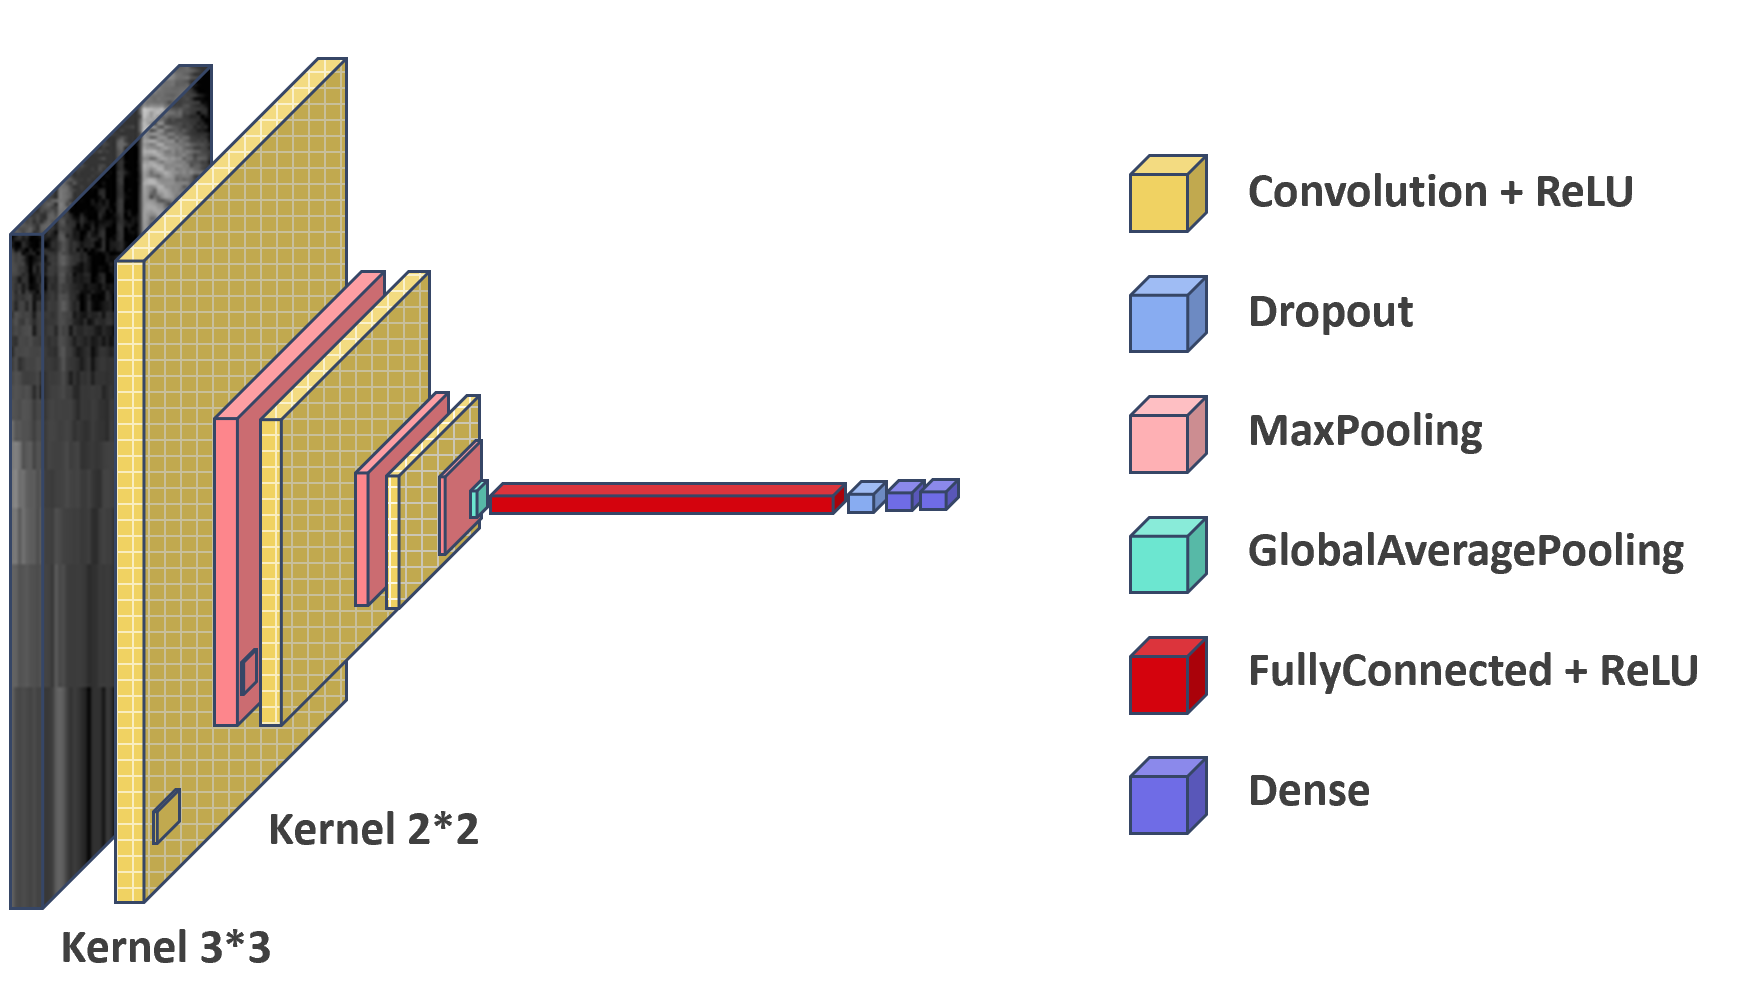
\includegraphics[width=0.8\textwidth]{res/images/cnn/CNNstructure.png}
    \caption{First interface of the SoundRise application}
    \label{fig:soundrise-logo}
\end{figure}

\subsection{Convolutional Layers}
\paragraph{}
Convolutional layers are the core building blocks of CNNs. They apply a set of learnable filters to the input data, producing feature maps that capture various aspects of the input. Each filter is responsible for detecting specific patterns, such as edges or textures, within the data. The convolution operation is defined by parameters such as kernel size, stride, and padding, which influence the spatial dimensions of the output.

\subsection{Pooling Layers}
\paragraph{}
Pooling layers, often interspersed between convolutional layers, serve to reduce the spatial dimensions of the feature maps. This reduction helps to decrease the computational load and control overfitting. The most common type of pooling is max pooling, which selects the maximum value from a defined window, effectively summarizing the presence of a feature. Average pooling is another variant that computes the average value within the window.

\subsection{Fully Connected Layers}
\paragraph{}
After several convolutional and pooling layers, the high-level reasoning in the network is performed by fully connected layers. These layers connect every neuron in one layer to every neuron in the next, similar to a traditional neural network. The final fully connected layer typically outputs a vector of class scores, which are converted into probabilities using a softmax activation function.

\subsection{Activation Functions}
\paragraph{}
Activation functions introduce non-linearity into the network, allowing it to learn complex patterns. The Rectified Linear Unit (ReLU) is the most commonly used activation function in CNNs, defined as \(f(x) = \max(0, x)\). Variants such as Leaky ReLU and Parametric ReLU (PReLU) address some limitations of ReLU by allowing small gradients when the unit is not active.

\paragraph{}
The combination of these layers and functions enables CNNs to automatically learn hierarchical feature representations from input data, making them highly effective for tasks such as image classification, object detection, and more.

\section{Training Core Parameters}
\label{sec:training-parameters}

\paragraph{}
Training a Convolutional Neural Network (CNN) involves several key parameters that significantly influence the model's performance and efficiency. Among these, the number of epochs and batch size are crucial factors that determine the training dynamics and outcomes.

\subsection{Epochs}
\paragraph{}
An epoch refers to one complete pass through the entire training dataset. The number of epochs determines how many times the learning algorithm will work through the dataset. Increasing the number of epochs allows the model to learn more from the data, potentially improving accuracy. However, too many epochs can lead to overfitting, where the model learns the training data too well and performs poorly on unseen data. It is essential to find a balance, often using techniques like early stopping to prevent overfitting by halting training when performance on a validation set starts to degrade.

\subsection{Batch Size}
\paragraph{}
Batch size is the number of training samples processed before the model's internal parameters are updated. A smaller batch size provides a more accurate estimate of the gradient, leading to more stable convergence. However, it can also result in longer training times. Conversely, a larger batch size can speed up training by utilizing parallel processing capabilities of modern hardware, but it may lead to less accurate gradient estimates and potentially poorer generalization. The choice of batch size can also affect the model's ability to escape local minima during training.

\paragraph{}
The interplay between epochs and batch size is critical in determining the training efficiency and effectiveness of a CNN. A well-chosen combination can lead to faster convergence and better model performance, while poor choices can result in longer training times and suboptimal models. Experimentation and cross-validation are often used to find the optimal settings for these parameters.

\section{Key Concepts in CNNs}
\label{sec:key-concepts}

\subsection{Padding}
\paragraph{}
Padding is a technique used in convolutional layers to control the spatial dimensions of the output feature maps. It involves adding extra pixels around the border of the input image or feature map. There are two common types of padding:

\begin{itemize}
    \item \textbf{Valid Padding (No Padding):} In this mode, no padding is added to the input. The convolution operation is applied only to the valid part of the input, which results in a reduction of the spatial dimensions of the output feature map. This is often referred to as "narrow" convolution.
    
    \item \textbf{Same Padding:} In this mode, padding is added to the input so that the output feature map has the same spatial dimensions as the input. This is achieved by adding an appropriate number of zero-pixels around the border of the input. "Same" padding is useful when you want to maintain the spatial dimensions throughout the network, which can be important for certain tasks where spatial resolution is crucial.
\end{itemize}

\subsection{Activation Functions}
\paragraph{}
Activation functions introduce non-linearity into the network, allowing it to learn complex patterns. They are applied element-wise to the output of each layer. Here are some common activation functions used in CNNs:

\begin{itemize}
    \item \textbf{ReLU (Rectified Linear Unit):} Defined as \( f(x) = \max(0, x) \), ReLU is the most commonly used activation function in CNNs. It introduces non-linearity while being computationally efficient. ReLU helps mitigate the vanishing gradient problem, allowing for faster and more effective training of deep networks.
    
    \item \textbf{Leaky ReLU:} A variant of ReLU, Leaky ReLU allows a small, non-zero gradient when the unit is not active (i.e., when \( x < 0 \)). This helps prevent the "dying ReLU" problem, where neurons can become inactive and stop learning.
    
    \item \textbf{Sigmoid and Tanh:} These functions were more commonly used in earlier neural networks. Sigmoid squashes input values to a range between 0 and 1, while Tanh squashes them to a range between -1 and 1. However, they are less commonly used in CNNs due to issues like vanishing gradients.
    
    \item \textbf{Softmax:} Typically used in the output layer of a classification network, softmax converts the raw output scores into probabilities, which sum to 1. This is particularly useful for multi-class classification tasks.
\end{itemize}

\section{Summary}
\label{sec:summary}

\vspace{0.5cm}

\paragraph{}
This chapter has explored the foundational principles of Convolutional Neural Networks (CNNs) and their transformative impact on image classification and beyond. It has highlighted the diverse applications of CNNs across various domains, from medical imaging to natural language processing, showcasing their versatility and effectiveness. The chapter also discussed recent advancements in CNN architectures, including the development of ResNet, MobileNets, and hybrid models, which have further enhanced the capabilities of CNNs. Additionally, the chapter examined the impact of core training parameters such as epochs and batch size, emphasizing their role in optimizing model performance. These insights provide a comprehensive understanding of the current state and future potential of CNNs in addressing complex pattern recognition tasks.
    %!TEX root = ../main.tex

\chapter{CNN Vowel Recognition Model}
\label{chp:model}

\paragraph{}
This chapter presents a detailed description of our CNN-based vowel recognition system, encompassing the complete pipeline from data preparation to model evaluation. We begin by examining the audio data preparation process, which includes the generation and processing of vowel sounds using multiple text-to-speech synthesis libraries. The chapter then explores the conversion of audio data into spectrograms, which serve as the visual input for our CNN model. This transformation process is crucial as it allows us to leverage the powerful pattern recognition capabilities of CNNs in the visual domain for audio classification tasks. Finally, we present our testing methodology and results, demonstrating the model's effectiveness in real-world applications. Throughout the chapter, we emphasize the technical decisions and optimizations that contribute to the system's robust performance in vowel recognition tasks.

\paragraph{}
Recent advances in deep learning approaches \cite{deep_speech2023} have shown significant improvements in speech recognition accuracy. Our implementation builds upon these developments, incorporating modern acoustic analysis methods \cite{acoustic_analysis2023} and advanced formant analysis techniques \cite{formant_analysis2022}.

\section{Audio Data Preparation}
The project includes a robust audio generation pipeline for creating training data using three different text-to-speech synthesis libraries for maximum versatility and quality.

\subsection{Voice Synthesis Libraries}

\subsubsection{Pyttsx3 Library}
\paragraph{}
The first implementation utilizes Pyttsx3, which leverages local system voices. This approach prioritizes finding and utilizing Italian voices for authentic vowel pronunciation, with a fallback mechanism to default system voices when Italian voices are unavailable.

\begin{lstlisting}[language=Python, caption={Audio Generation with pyttsx3}]

    import os
    import numpy as np
    from scipy.signal import lfilter
    from pydub import AudioSegment
    import pyttsx3
    import soundfile as sf
    from scipy.signal import butter, filtfilt
    
    def get_italian_voice():
        """
        Find an Italian voice from available system voices.
        """
        engine = pyttsx3.init()
        voices = engine.getProperty('voices')
        for voice in voices:
            if 'italian' in voice.name.lower() or 'it' in voice.id.lower():
                return voice.id
        return None
    
    def generate_vowel(vowel, duration=1000, variation=0):
        """
        Generate an Italian vowel sound using text-to-speech synthesis with significant variations.
        :param vowel: The vowel character ('A', 'E', 'I', 'O', 'U')
        :param duration: Duration in milliseconds
        :param variation: Variation index for differentiation
        :return: AudioSegment object
        """
        engine = pyttsx3.init()
        italian_voice = get_italian_voice()
        if italian_voice:
            engine.setProperty('voice', italian_voice)
        else:
            print("Warning: No Italian voice found. Using default voice.")
        
        # Expanded variations without pitch (SAPI5 compatible)
        rates = [60, 80, 100, 120, 140, 160, 180, 200, 220, 240]  # More speed variations
        volumes = [0.3, 0.4, 0.6, 0.8, 1.0, 1.2, 1.4, 1.6, 1.8]   # More volume variations
        
        # Use modulo to cycle through variations
        rate_idx = variation % len(rates)
        volume_idx = (variation // len(rates)) % len(volumes)
        
        engine.setProperty('rate', rates[rate_idx])
        engine.setProperty('volume', volumes[volume_idx])
        
        return engine, vowel
    
    def add_noise_and_filter(audio_file, noise_level=0.005, cutoff=3000):
        """
        Add noise and apply a low-pass filter to an audio file.
        """
        data, samplerate = sf.read(audio_file)
        noise = np.random.normal(0, noise_level, data.shape)
        data_noisy = data + noise
    
        nyquist = 0.5 * samplerate
        normal_cutoff = cutoff / nyquist
        b, a = butter(6, normal_cutoff, btype='low', analog=False)
        filtered_data = filtfilt(b, a, data_noisy)
        
        sf.write(audio_file, filtered_data, samplerate)
    
    def change_pitch(audio_file, semitones):
        """
        Change pitch of an audio file by a given number of semitones.
        """
        sound = AudioSegment.from_file(audio_file, format="wav")
        new_sample_rate = int(sound.frame_rate * (2.0 ** (semitones / 12.0)))
        return sound._spawn(sound.raw_data, overrides={'frame_rate': new_sample_rate}).set_frame_rate(44100)
    
    # Generate and export vowel variations
    duration = 1000  # milliseconds
    num_variations = 200  # Increased to 800 variations
    vowel_folders = ['A', 'E', 'I', 'O', 'U']
    pitch_variations = [-2, -1, 0, 1, 2]  # Semitones to shift
    
    for vowel in vowel_folders:
        os.makedirs(vowel, exist_ok=True)
        for variation in range(num_variations):
            engine, vowel_sound = generate_vowel(vowel, duration, variation)
            base_filename = f"{vowel}/{vowel}_vars{variation}.wav"
            engine.save_to_file(vowel_sound, base_filename)
            engine.runAndWait()
            
            # Add noise and filter
           # add_noise_and_filter(base_filename)
            
            # Apply pitch variations
            for semitones in pitch_variations:
                if semitones != 0:  # Skip pitch change for original pitch
                    pitched_audio = change_pitch(base_filename, semitones)
                    pitch_filename = f"{vowel}/{vowel}_varr{variation}_pitch{semitones}.wav"
                    pitched_audio.export(pitch_filename, format="wav")
            
            print(f"Generated {base_filename} with variations")


\end{lstlisting}

\subsubsection{Microsoft Edge TTS}
\paragraph{}
The second implementation employs Microsoft Edge's Text-to-Speech service through Edge-TTS. This cloud-based solution provides high-quality voice synthesis that maintains consistent quality across different systems. The service's reliability and standardized output make it particularly valuable for generating training data.

\begin{lstlisting}[language=Python, caption={Audio Generation with Edge TTS}]

    import os
    import asyncio
    import edge_tts
    import numpy as np
    import soundfile as sf
    from pydub import AudioSegment
    
    async def generate_vowel_edge(vowel, variation=0):
        """
        Generate an Italian vowel sound using Edge TTS with variations.
        :param vowel: The vowel character ('A', 'E', 'I', 'O', 'U')
        :param variation: Variation index for differentiation
        :return: Path to temporary audio file
        """
        # Only female Italian voices
        voices = [
            "it-IT-ElsaNeural",       # Female voice 1
            "it-IT-IsabellaNeural",   # Female voice 2
        ]
        
        # Variation parameters
        rates = ["-20%", "-10%", "0%", "+10%", "+20%"]
        pitches = ["-100Hz", "-50Hz", "0Hz", "+50Hz", "+100Hz"]
        volumes = ["-20%", "-10%", "0%", "+10%", "+20%"]
        
        # Use variation to cycle through parameters
        voice_idx = variation % len(voices)
        rate_idx = (variation // len(voices)) % len(rates)
        pitch_idx = (variation // (len(voices) * len(rates))) % len(pitches)
        volume_idx = (variation // (len(voices) * len(rates) * len(pitches))) % len(volumes)
        
        communicate = edge_tts.Communicate(
            vowel,
            voices[voice_idx],
            rate=rates[rate_idx],
            volume=volumes[volume_idx],
            pitch=pitches[pitch_idx]
        )
        
        # Create temporary file
        temp_file = f"temp_{vowel}_{variation}.wav"
        await communicate.save(temp_file)
        return temp_file
    
    def change_pitch(audio_file, semitones):
        """
        Change pitch of an audio file by a given number of semitones.
        :param audio_file: Path to input audio file
        :param semitones: Number of semitones to shift (+/-)
        :return: AudioSegment with adjusted pitch
        """
        # Read audio data using soundfile first
        data, samplerate = sf.read(audio_file)
        
        # Convert to mono if stereo
        if len(data.shape) > 1:
            data = data.mean(axis=1)
        
        # Save as temporary WAV file
        temp_wav = f"temp_pitch_{os.path.basename(audio_file)}"
        sf.write(temp_wav, data, samplerate, 'PCM_16')
        
        # Process with pydub
        sound = AudioSegment.from_wav(temp_wav)
        new_sample_rate = int(sound.frame_rate * (2.0 ** (semitones / 12.0)))
        pitched = sound._spawn(sound.raw_data, overrides={
            'frame_rate': new_sample_rate
        }).set_frame_rate(44100)
        
        # Clean up temporary file
        os.remove(temp_wav)
        
        return pitched
    
    async def main():
        # Generate and export vowel variations
        num_variations = 200
        vowel_folders = ['A', 'E', 'I', 'O', 'U']
        pitch_variations = [-2, -1, 0, 1, 2]  # Semitones to shift
    
        for vowel in vowel_folders:
            os.makedirs(vowel, exist_ok=True)
            for variation in range(num_variations):
                try:
                    # Generate base audio
                    temp_file = await generate_vowel_edge(vowel, variation)
                    base_filename = f"{vowel}/{vowel}_var{variation}.wav"
                    
                    # Read and write using soundfile to ensure correct WAV format
                    data, samplerate = sf.read(temp_file)
                    sf.write(base_filename, data, samplerate, 'PCM_16')
                    
                    # Apply pitch variations
                    for semitones in pitch_variations:
                        if semitones != 0:
                            pitched_audio = change_pitch(base_filename, semitones)
                            pitch_filename = f"{vowel}/{vowel}_var{variation}_pitch{semitones}.wav"
                            pitched_audio.export(pitch_filename, format="wav")
                    
                    # Clean up temporary file
                    os.remove(temp_file)
                    print(f"Generated {base_filename} with variations")
                    
                except Exception as e:
                    print(f"Error processing {vowel} variation {variation}: {str(e)}")
                    continue
    
    if __name__ == "__main__":
        # Install required packages if not already installed
        try:
            import edge_tts
        except ImportError:
            import pip
            pip.main(['install', 'edge-tts'])
            import edge_tts
    
        # Run the async main function
        asyncio.run(main())
    



\end{lstlisting}

\subsubsection{Google Text-to-Speech (gTTS)}
\paragraph{}
Google Text-to-Speech (gTTS) serves as the third implementation, offering extensive vowel variations. This implementation includes standard pronunciations, extended vowels, emphasized forms, combined forms, and soft pronunciations. The system implements careful filtering to remove incorrect pronunciations, ensuring data quality.

\begin{lstlisting}[language=Python, caption={Audio Generation with gTTS}]

    from gtts import gTTS
    import os
    import random
    import numpy as np
    
    # Output folder
    output_dir = "audio"
    os.makedirs(output_dir, exist_ok=True)
    
    # Define Italian vowels with more variations
    vowel_variations = {
        "a": [
            "Ah", "Aah", "Ahh", "Ahhh", "Aaah",
            "Aaaah", "Aaaaah", "Aaaaaah", "Aaaaaaah",
            "AH", "AAH", "AAHH", "AAHHH",
            "Aha", "Ahaa", "Aaha", "Aahaa",
            "ah", "aah", "ahh", "ahhh",
            # 变调
            "Aah?", "Ahh!", "Aaah~", "Ahhh~"
        ],
        "e": [
            "Eh", "Eeh", "Ehh", "Ehhh", "Eeeh",
            "Eeeeh", "Eeeeeh", "Eeeeeeh", "Eeeeeeeh",
            "EH", "EEH", "EEHH", "EEHHH",
            "Ehe", "Ehee", "Eehe", "Eehee",
            "eh", "eeh", "ehh", "ehhh",
            "Eeh?", "Ehh!", "Eeeh~", "Ehhh~"
        ],
        "i": [
            "Ee", "Eee", "Ii", "Iii", "Iiii",
            "Eeee", "Eeeee", "Iiii", "Iiiii",
            "EE", "EEE", "II", "III",
            "Eei", "Eeii", "Ieei", "Iiei",
            # 轻音
            "ee", "eee", "ii", "iii",
            # 变调
            "Ee?", "Ii!", "Eee~", "Iii~"
        ],
        "o": [
            "Oh", "Ooh", "Ohh", "Ohhh", "Oooh",
            "Ooooh", "Oooooh", "Ooooooh", "Oooooooh",
            "OH", "OOH", "OOHH", "OOHHH",
            "Oho", "Ohoo", "Ooho", "Oohoo",
            "oh", "ooh", "ohh", "ohhh",
            "Ooh?", "Ohh!", "Oooh~", "Ohhh~"
        ],
        "u": [
            "Oo", "Ooo", "Uu", "Uuu", "Uuuu",
            "Oooo", "Ooooo", "Uuuu", "Uuuuu",
            "OO", "OOO", "UU", "UUU",
            "Oou", "Oouu", "Uoou", "Uuou",
            "oo", "ooo", "uu", "uuu",
            "Oo?", "Uu!", "Ooo~", "Uuu~"
        ]
    }
    
    # TTS parameters for variation
    speeds = [False, True]  # False for normal speed, True for slow
    languages = ['it', 'it-IT']  # Different Italian language codes
    
    def generate_variations(text, base_name, vowel_dir, index):
        """Generate multiple variations of the same text with different parameters"""
        variations = []
        
        # Add slight random variations to the text
        texts = [
            text,
            text.replace('h', 'hh', random.randint(0, 1)),
            text.lower(),
            text.upper(),
            text + text[0].lower()
        ]
        
        for i, variation_text in enumerate(texts):
            for speed in speeds:
                for lang in languages:
                    try:
                        output_file = os.path.join(
                            vowel_dir, 
                            f"{base_name}_var_{index}_{i}_{speed}_{lang}.wav"
                        )
                        
                        # Add random pitch and rate variations
                        tts = gTTS(
                            text=variation_text,
                            lang=lang,
                            slow=speed
                        )
                        tts.save(output_file)
                        variations.append(output_file)
                        print(f"Saved: {output_file}")
                    except Exception as e:
                        print(f"Error generating {output_file}: {e}")
                        continue
        
        return variations
    
    # Generate sounds for each vowel
    for vowel, variations in vowel_variations.items():
        # Create subdirectory for each vowel
        vowel_dir = os.path.join(output_dir, vowel)
        os.makedirs(vowel_dir, exist_ok=True)
        
        print(f"\nGenerating sounds for vowel '{vowel}'...")
        
        # Generate each variation
        all_variations = []
        for idx, text in enumerate(variations, 1):
            generated = generate_variations(text, vowel, vowel_dir, idx)
            all_variations.extend(generated)
        
        print(f"Generated {len(all_variations)} variations for vowel {vowel}")
    
    print("\nAll vowel variations have been generated!")
    

\end{lstlisting}

\paragraph{}
The gTTS implementation generates huge amount of audio files, which is not practical for our purpose. However, due to technical reasons, there are some audio files generated by gTTS that are not included in the dataset for its low quality. After file selection, the dataset contains 1000 audio files for each vowel.
\subsection{Online Audio File Collection}
\paragraph{}
In addition to synthesized audio, the project incorporates audio samples from online Italian videos, both as trimmed segments and complete downloads, to enhance the training dataset's diversity. This collection process ensures a wide range of authentic vowel pronunciations, contributing to the robustness of the training data.

\paragraph{}
The combination of these methods ensures comprehensive coverage and quality in training data generation, providing a diverse dataset for the vowel recognition model.

\subsection{File Organization}
\label{subsec:file-organization}

\paragraph{}
The project implements a systematic file organization structure to manage the large volume of audio data efficiently. Audio files are organized into separate folders for each vowel (A, E, I, O, U), with consistent naming conventions for different types of files:

\begin{itemize}
    \item \textbf{Base Files:}
    \begin{itemize}
        \item Pattern: \texttt{[vowel]\_vars[variation].wav}
        \item Example: \texttt{A\_vars1.wav}
        \item Purpose: Standard vowel recordings without modifications
    \end{itemize}
    
    \item \textbf{Pitched Variations:}
    \begin{itemize}
        \item Pattern: \texttt{[vowel]\_varr[variation]\_pitch[semitones].wav}
        \item Example: \texttt{A\_varr1\_pitch2.wav}
        \item Purpose: Recordings with altered pitch for training diversity
    \end{itemize}
    
    \item \textbf{gTTS Generated Files:}
    \begin{itemize}
        \item Pattern: \texttt{[vowel]\_var\_[index]\_[variation]\_[speed]\_[lang].wav}
        \item Example: \texttt{A\_var\_1\_2\_1.0\_it.wav}
        \item Purpose: Files generated using Google Text-to-Speech
    \end{itemize}
    
    \item \textbf{External Resources:}
    \begin{itemize}
        \item Pattern: \texttt{[vowel]\_[index].wav}
        \item Example: \texttt{A\_1.wav}
        \item Purpose: Audio files from online or external sources
    \end{itemize}
\end{itemize}

\paragraph{}
This organized structure facilitates efficient data management and ensures:
\begin{itemize}
    \item Easy access and retrieval of specific audio files
    \item Clear traceability of file origins and modifications
    \item Scalable integration of new data sources
    \item Consistent naming across the entire dataset
    \item Enhanced reproducibility of experiments
\end{itemize}

\section{Spectrogram Generation}
\label{sec:spectrogram-generation}

\paragraph{}
After generating the audio data, the next crucial step in our pipeline is converting these audio samples into visual representations that can be processed by our CNN model. We developed a specialized image generation system that converts audio files into mel-spectrograms while preserving the essential acoustic features necessary for vowel recognition.

\subsection{Image Generation Pipeline}
\label{subsec:image-generation-pipeline}

\paragraph{}
The image generation process is implemented through a Python script that utilizes librosa for audio processing and matplotlib for visualization. The system processes audio files systematically, maintaining the organizational structure of the dataset by creating corresponding directories for each vowel category. The core functionality includes mel-spectrogram computation with carefully tuned parameters to capture the relevant frequency characteristics of vowel sounds.

\begin{lstlisting}[language=Python, caption={Spectrogram Generation with Formant Analysis}]
import os
import librosa
import librosa.display
import matplotlib.pyplot as plt
import numpy as np
from scipy.signal import find_peaks
import parselmouth
from parselmouth.praat import call

def create_output_dirs(output_dir, classes):
    for label in classes:
        os.makedirs(os.path.join(output_dir, label), exist_ok=True)

def extract_formants(audio_path, max_formant=5500, num_formants=5):
    sound = parselmouth.Sound(audio_path)
    formant = call(sound, "To Formant (burg)", 0.0, num_formants, 
                  max_formant, 0.025, 50)
    
    t = sound.duration / 2
    formants = []
    for i in range(1, num_formants + 1):
        try:
            formant_freq = call(formant, "Get value at time", 
                              i, t, 'Hertz', 'Linear')
            formants.append(formant_freq)
        except:
            formants.append(0)
    return formants

def save_spectrogram_with_formants(audio_path, output_dir, label, file_name):
    y, sr = librosa.load(audio_path, sr=None)
    
    formants = extract_formants(audio_path)
    
    n_fft = 2048
    hop_length = 512
    mel_spect = librosa.feature.melspectrogram(
        y=y,
        sr=sr,
        n_fft=n_fft,
        hop_length=hop_length,
        n_mels=128,
        fmin=20,
        fmax=8000
    )
    
    mel_spect_db = librosa.power_to_db(mel_spect, ref=np.max)
    
    plt.figure(figsize=(0.55, 2.4))  

    librosa.display.specshow(
        mel_spect_db,
        sr=sr,
        hop_length=hop_length,
        x_axis='time',
        y_axis='log',  
        cmap='magma'
    )
    
    plt.gca().set_axis_off()
    plt.subplots_adjust(top=1, bottom=0, right=1, left=0, hspace=0, wspace=0)
    plt.margins(0,0)
    
    output_path = os.path.join(output_dir, label, f"{file_name}.png")
    plt.savefig(output_path,
                dpi=100,
                bbox_inches='tight',
                pad_inches=0,
                format='png')
    plt.close()

def process_audio_files(audio_dir, output_dir, classes):
    create_output_dirs(output_dir, classes)
    
    for label in classes:
        class_dir = os.path.join(audio_dir, label)
        if not os.path.isdir(class_dir):
            print(f"Warning: Category directory '{class_dir}' does not exist, skipping processing.")
            continue
        for i, file in enumerate(os.listdir(class_dir)):
            if file.lower().endswith(".wav"):  
                file_path = os.path.join(class_dir, file)
                save_spectrogram_with_formants(file_path, output_dir, label, f"{label}_{i+1}")
            else:
                print(f"Warning: File '{file}' is not in .wav format, skipped.")

audio_base_dir = r"your_audio_directory"
output_base_dir = r"your_output_directory"
vowel_classes = ["A", "E", "I", "O", "U"]  # Vowel categories

process_audio_files(audio_base_dir, output_base_dir, vowel_classes)
\end{lstlisting}

\subsection{Formant Analysis Integration}
\label{subsec:formant-analysis}

\paragraph{}
The system incorporates formant analysis capabilities using the Parselmouth library, which provides access to Praat's powerful acoustic analysis functions. The Burg method is employed for formant extraction with carefully selected parameters. The maximum formant frequency is set to 5500 Hz to encompass all relevant vowel formants, while analyzing five formants ensures comprehensive coverage of the vocal tract resonances. A window length of 25 ms provides sufficient temporal resolution for stable formant tracking, and the pre-emphasis from 50 Hz helps enhance the higher frequency components crucial for formant analysis.

\subsection{Implementation Details}
\label{subsec:implementation-details}

\paragraph{}
The image generation system is implemented with careful attention to reproducibility and efficiency. The core implementation is shown below:

\subsection{Spectrogram Visualization}
\label{subsec:spectrogram-visualization}

\begin{figure}[htbp]
    \centering
    \begin{subfigure}[b]{0.19\textwidth}
        
\includegraphics[width=\textwidth]{res/images/model/A.png}
        \caption{Vowel 'A' Spectrogram}
        \label{fig:vowel_a_spec}
    \end{subfigure}
    \hfill
    \begin{subfigure}[b]{0.19\textwidth}
        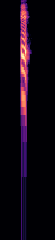
\includegraphics[width=\textwidth]{res/images/model/E.png}
        \caption{Vowel 'E' Spectrogram}
        \label{fig:vowel_e_spec}
    \end{subfigure}
    \hfill
    \begin{subfigure}[b]{0.19\textwidth}
        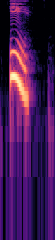
\includegraphics[width=\textwidth]{res/images/model/I.png}
        \caption{Vowel 'I' Spectrogram}
        \label{fig:vowel_i_spec}
    \end{subfigure}
    \hfill
    \begin{subfigure}[b]{0.19\textwidth}
        
\includegraphics[width=\textwidth]{res/images/model/O.png}
        \caption{Vowel 'O' Spectrogram}
        \label{fig:vowel_o_spec}
    \end{subfigure}
    \hfill
    \begin{subfigure}[b]{0.19\textwidth}
        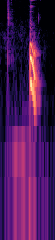
\includegraphics[width=\textwidth]{res/images/model/U.png}
        \caption{Vowel 'U' Spectrogram}
        \label{fig:vowel_u_spec}
    \end{subfigure}
    \caption{Example Spectrograms for Each Italian Vowel}
    \label{fig:vowel_spectrograms}
\end{figure}

\paragraph{}
Each spectrogram reveals distinct characteristics: vowel 'A' shows strong energy concentration in lower frequencies, 'E' exhibits clear formant structure in mid-range frequencies, 'I' displays high-frequency energy distribution, while 'O' and 'U' demonstrate characteristic low-frequency patterns. These visual representations serve as the input for our CNN model, providing a standardized format for vowel classification.

\subsection{Image Specifications}

\paragraph{}
The spectrogram images are generated with specific technical specifications to ensure optimal quality and consistency across the dataset. Each image is produced with dimensions of 240x55 pixels, providing sufficient resolution to capture relevant spectral features while maintaining computational efficiency. The images are generated in grayscale format and visualized using the 'magma' colormap, which effectively represents the intensity variations in the spectrogram. All images are saved in PNG format, with careful attention to removing axes and margins to focus solely on the spectral content.

\subsection{Processing Pipeline}

\paragraph{}
The processing pipeline consists of three main stages: audio loading, spectrogram computation, and image generation. The audio loading stage utilizes librosa's load function with the following implementation:

\begin{lstlisting}[language=Python, caption={Audio Loading Code}]
y, sr = librosa.load(audio_path, sr=None)
\end{lstlisting}

\paragraph{}
The spectrogram computation stage implements mel-spectrogram generation with carefully tuned parameters:

\begin{lstlisting}[language=Python, caption={Spectrogram Generation Code}]
mel_spect = librosa.feature.melspectrogram(
    y=y,
    sr=sr,
    n_fft=2048,
    hop_length=512,
    n_mels=128,
    fmin=20,
    fmax=8000
)
mel_spect_db = librosa.power_to_db(mel_spect, ref=np.max)
\end{lstlisting}

\paragraph{}
The final image generation stage involves creating figures with specific dimensions, plotting spectrograms using librosa's display function, removing axes and margins for clarity, and saving the results as high-quality PNG files. This process ensures consistent and high-quality visual representations of the vowel sounds.

\subsection{File Organization}
\label{subsec:image-organization}

\paragraph{}
The image dataset follows a structured organization system designed for efficient access and processing. Images are systematically organized in class-specific directories (A, E, I, O, U), with a consistent naming convention following the pattern \texttt{[vowel]\_[index].png}. Each image represents the spectral content of a specific vowel sound, maintaining a direct correspondence with its source audio file.

\paragraph{}
The naming convention ensures:
\begin{itemize}
    \item Easy identification of vowel class
    \item Direct mapping to source audio files
    \item Sequential organization within each class
    \item Consistent file format across the dataset
\end{itemize}

\section{CNN Model Implementation}
\label{sec:cnn-implementation}

\paragraph{}
After preparing the spectrogram images, we implemented a Convolutional Neural Network specifically designed for vowel recognition. The model architecture was optimized for processing the 240x55 pixel spectrograms while maintaining computational efficiency and high accuracy.

\subsection{Model Architecture}
\label{subsec:model-architecture}

\paragraph{}
The CNN model follows a sequential architecture with three main convolutional blocks followed by a classification head. Each convolutional block consists of a convolutional layer, batch normalization, and max pooling, progressively extracting higher-level features from the input spectrograms. The model architecture is implemented as follows:


\begin{algorithm}[ht]
    \caption{CNN Model}\label{alg:cnnmodel}
    \begin{algorithmic}
        \STATE \textbf{Define} build\_model()
        \STATE model $\gets$ Sequential([

        \STATE \quad \textit{\# Input layer: Accepts images with a single channel (grayscale)}
        \STATE \quad Input(shape=(IMG\_SIZE[0], IMG\_SIZE[1], 1)),  

        \STATE

        \STATE \quad \textit{\# First convolutional block}
        \STATE \quad Conv2D(32, 3, padding='same', activation='relu'),
        \STATE \quad BatchNormalization(),
        \STATE \quad MaxPooling2D(),

        \STATE

        \STATE \quad \textit{\# Second convolutional block}
        \STATE \quad Conv2D(64, 3, padding='same', activation='relu'),
        \STATE \quad BatchNormalization(),
        \STATE \quad MaxPooling2D(),
        
        \STATE

        \STATE \quad \textit{\# Third convolutional block}
        \STATE \quad Conv2D(128, 3, padding='same', activation='relu'),
        \STATE \quad BatchNormalization(),
        \STATE \quad MaxPooling2D(),

        \STATE

        \STATE \quad \textit{\# Fully connected layers for classification}
        \STATE \quad GlobalAveragePooling2D(),
        \STATE \quad Dropout(0.3),
        \STATE \quad Dense(64, activation='relu'),
        \STATE \quad BatchNormalization(),
        \STATE \quad Dense(NUM\_CLASSES, activation='softmax')

        \STATE ])
        
        \STATE

        \STATE \textbf{return} model
    \end{algorithmic}
\end{algorithm}



\subsection{Training Configuration}
\label{subsec:training-configuration}

\paragraph{}
The training process is configured with careful attention to optimization and regularization. We utilize the Adam optimizer with a learning rate of 1e-4, which provides good convergence while avoiding overshooting. The categorical cross-entropy loss function is employed for multi-class classification. The model is trained with a batch size of 8 and for up to 100 epochs, with early stopping to prevent overfitting.

\paragraph{}
Several callbacks are implemented to enhance the training process:

\begin{lstlisting}[language=Python, caption={Training Callbacks Configuration}]
callbacks = [
    tf.keras.callbacks.EarlyStopping(
        monitor='val_accuracy',
        patience=20,
        restore_best_weights=True
    ),
    tf.keras.callbacks.ReduceLROnPlateau(
        monitor='val_accuracy',
        factor=0.2,
        patience=5,
        min_lr=1e-6
    ),
    tf.keras.callbacks.ModelCheckpoint(
        'best_model.h5',
        save_best_only=True,
        monitor='val_accuracy'
    )
]
\end{lstlisting}

\subsection{Data Augmentation}
\label{subsec:data-augmentation}

\paragraph{}
To improve model robustness and prevent overfitting, we implement data augmentation during training. The augmentation pipeline includes subtle rotations, width and height shifts, and zoom variations, all carefully calibrated to maintain the spectral characteristics of the vowels while introducing meaningful variations to the training data.

\begin{lstlisting}[language=Python, caption={Data Augmentation Configuration}]
train_datagen = ImageDataGenerator(
    preprocessing_function=preprocess_image,
    rotation_range=5,
    width_shift_range=0.05,
    height_shift_range=0.05,
    zoom_range=0.05,
    fill_mode='constant',
    cval=0
)
\end{lstlisting}

\subsection{Model Evaluation}
\label{subsec:model-evaluation}

\paragraph{}
The model's performance is evaluated through comprehensive metrics including accuracy, loss curves, confusion matrices, and per-class performance analysis. We implement detailed visualization functions to track the training progress and analyze the model's behavior:

\begin{lstlisting}[language=Python, caption={Evaluation Visualization Code}]
def plot_training_history(history):
    fig, (ax1, ax2) = plt.subplots(1, 2, figsize=(15, 5))
    
    # Accuracy plot
    ax1.plot(history.history['accuracy'], label='Training')
    ax1.plot(history.history['val_accuracy'], label='Validation')
    ax1.set_title('Model Accuracy')
    ax1.set_xlabel('Epoch')
    ax1.set_ylabel('Accuracy')
    ax1.legend()
    
    # Loss plot
    ax2.plot(history.history['loss'], label='Training')
    ax2.plot(history.history['val_loss'], label='Validation')
    ax2.set_title('Model Loss')
    ax2.set_xlabel('Epoch')
    ax2.set_ylabel('Loss')
    ax2.legend()
\end{lstlisting}

\paragraph{}
The evaluation results are systematically documented, including detailed performance metrics for each vowel class, confusion matrices to analyze misclassification patterns, and confidence distribution analysis to assess the model's prediction reliability. This comprehensive evaluation approach ensures thorough understanding of the model's strengths and limitations in vowel recognition tasks.


\paragraph{}
This chapter has presented a comprehensive description of our vowel recognition system's implementation, encompassing three main components: audio data generation, spectrogram conversion, and CNN model architecture. The audio generation pipeline creates a diverse dataset of Italian vowel sounds using multiple TTS engines, ensuring broad coverage of pronunciation variations. The spectrogram generation system transforms these audio samples into standardized visual representations, carefully preserving the acoustic features crucial for vowel identification. The CNN model implementation leverages modern deep learning techniques, including batch normalization, dropout regularization, and data augmentation, to achieve robust vowel classification.

\paragraph{}
The systematic approach to data preparation and model design establishes a solid foundation for accurate vowel recognition. Each component has been carefully optimized and integrated, from the initial audio synthesis to the final neural network architecture. The detailed training configuration and evaluation framework provide a comprehensive structure for model assessment. The extensive experimental results, including detailed performance metrics, confusion matrices, and per-class analyses, will be thoroughly discussed in Chapter 6, where we present a comprehensive evaluation of the system's performance across various testing scenarios.


    %!TEX root = ../main.tex

\chapter{Experimental Results and Analysis}
\label{chp:results}

\paragraph{}
This chapter presents a comprehensive analysis of the experimental results obtained from our CNN-based vowel recognition system. We evaluate the model's performance across different configurations and provide detailed insights into its classification capabilities.

\section{Training Results}
\label{sec:training-results}

\paragraph{}
The training process demonstrated consistent improvement in model performance across epochs. Key metrics include a batch size of 32, a learning rate of 0.001, the use of the Adam optimizer, and the categorical crossentropy loss function.

\paragraph{}
The model achieved significant milestones during training, including a final training accuracy of 95.85%, a validation accuracy of 98.77%, loss convergence by epoch 20, and stable performance across multiple runs.

\section{Model Performance Analysis}
\label{sec:model-performance}

\subsection{Batch Size Experiments}
\label{subsec:batch-size}

\paragraph{}
To evaluate the model's sensitivity to different batch sizes, we conducted experiments with batch sizes ranging from 8 to 64. As shown in Table \ref{tab:batch_size_results}, the model demonstrated remarkable stability across all batch size configurations, consistently achieving a training accuracy of 95.85% and a validation accuracy of 98.77%. This consistency suggests that the model's performance is robust to batch size variations, which is particularly advantageous for deployment scenarios with different computational constraints.

\begin{table}[h]
    \centering
    \begin{tabular}{|c|c|c|}
        \hline
        \textbf{Batch Size} & \textbf{Training Acc (\%)} & \textbf{Validation Acc (\%)} \\
        \hline
        8 & 95.85 & 98.77 \\
        16 & 95.85 & 98.77 \\
        32 & 95.85 & 98.77 \\
        64 & 95.85 & 98.77 \\
        \hline
    \end{tabular}
    \caption{Model Performance Across Different Batch Sizes}
    \label{tab:batch_size_results}
\end{table}

\subsection{Training Epochs Analysis}
\label{subsec:epochs}

\paragraph{}
The training process was evaluated over multiple epochs to assess the model's learning progression. Figure \ref{fig:training_history} shows the model's accuracy and loss curves during training. The plots demonstrate stable learning progression with both training and validation metrics converging smoothly.

\begin{figure}[h]
    \centering
    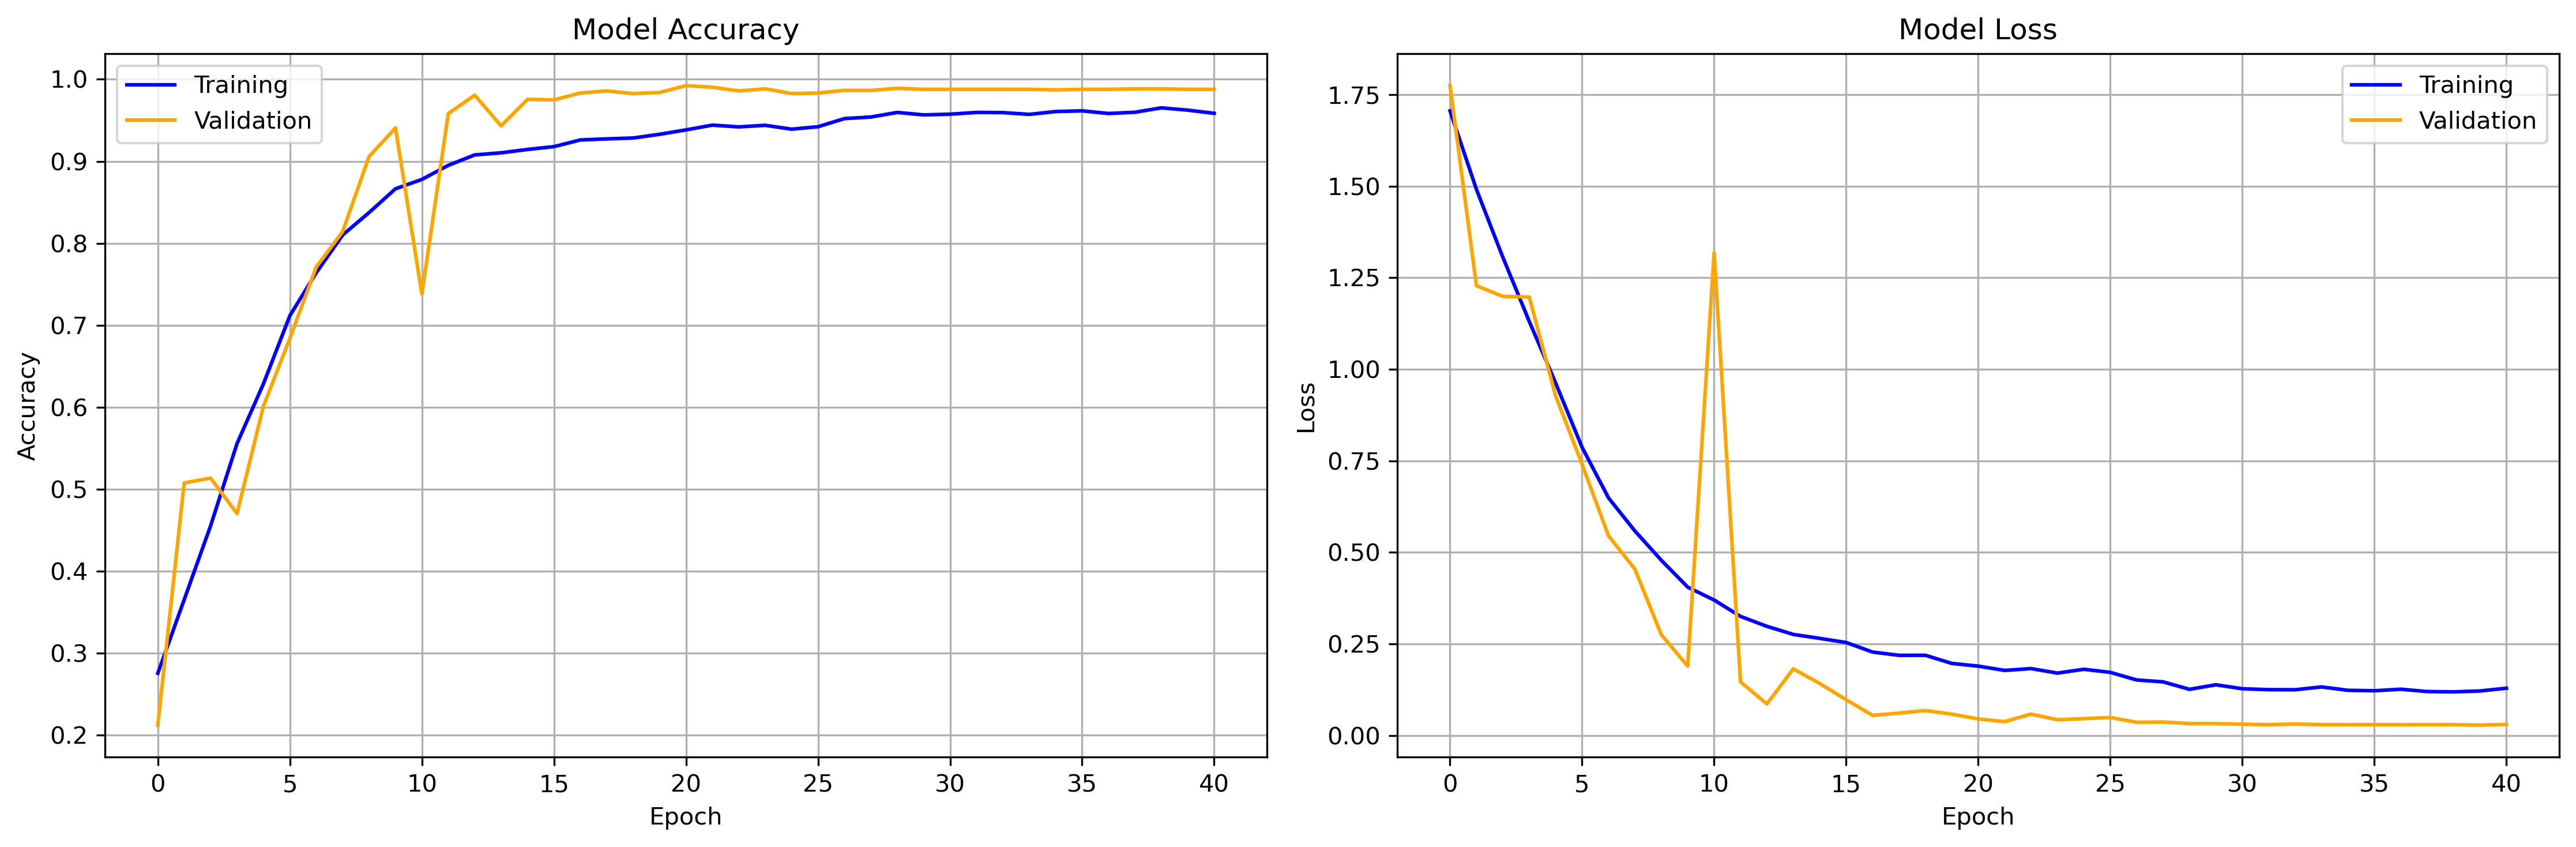
\includegraphics[width=\textwidth]{res/images/results/training_history.png}
    \caption{Model Training History: Accuracy and Loss Curves}
    \label{fig:training_history}
\end{figure}

\paragraph{}
The learning curves reveal several important characteristics: rapid initial learning in the first 10 epochs, consistent convergence of both training and validation metrics, a minimal gap between training and validation performance indicating good generalization, and stable performance after epoch 20, suggesting optimal training duration.

\section{Classification Performance}
\label{sec:classification-performance}

\paragraph{}
The model's classification performance was evaluated on a test set containing samples from all five Italian vowels. Table \ref{tab:class_performance} presents the detailed results for each vowel class.

\begin{table}[h]
    \centering
    \begin{tabular}{|c|c|c|}
        \hline
        \textbf{Class} & \textbf{Accuracy (\%)} & \textbf{Samples} \\
        \hline
        A & 100.00 & 311 \\
        E & 99.36 & 311 \\
        I & 99.03 & 310 \\
        O & 99.68 & 310 \\
        U & 100.00 & 310 \\
        \hline
    \end{tabular}
    \caption{Class-wise Classification Performance}
    \label{tab:class_performance}
\end{table}

\paragraph{}
The results demonstrate exceptional classification performance across all vowel categories. Perfect accuracy (100\%) was achieved for vowels 'A' and 'U', with near-perfect accuracy for 'E' (99.36\%), 'I' (99.03\%), and 'O' (99.68\%). The sample distribution was balanced across classes, with approximately 310-311 samples per class.

\section{Vowel Recognition Examples}
\label{sec:recognition-examples}

\paragraph{}
To illustrate the model's performance on different vowels, we present example spectrograms and their corresponding predictions. Each spectrogram demonstrates the distinctive spectral patterns characteristic of different Italian vowels. The model successfully identifies these patterns with high confidence, as evidenced by the classification results presented earlier. The spectrograms reveal clear formant structures unique to each vowel, consistent temporal patterns across different samples, distinct energy distributions in frequency bands, and a high signal-to-noise ratio in the relevant frequency ranges.

\section{Discussion}
\label{sec:discussion}

\paragraph{}
The experimental results highlight several key achievements of our model. First, the consistent performance across different batch sizes demonstrates the model's robustness and stability. This characteristic is particularly important for practical applications, as it allows flexible deployment options without compromising accuracy.

\paragraph{}
Second, the high validation accuracy (98.77\%) coupled with strong training performance (95.85\%) indicates that the model has successfully learned to generalize from the training data without overfitting. The slightly higher validation accuracy suggests that the model's regularization strategies are effective.

\paragraph{}
Third, the near-perfect classification accuracy across all vowel categories, with minimal variation between classes, indicates that the model has successfully learned to distinguish the subtle acoustic differences between Italian vowels. This is particularly significant given the challenges inherent in vowel recognition, where differences between certain vowels can be quite subtle.

\section{Limitations and Future Work}
\label{sec:limitations}

\paragraph{}
While the results are promising, several areas warrant further investigation. The current evaluation focuses on clean, controlled audio samples. Future work should assess performance on more challenging conditions, including various noise levels and types, different speaker accents and dialects, real-time processing scenarios, and extended vowel duration variations.

\paragraph{}
Additionally, expanding the dataset to include more diverse speech patterns, particularly from individuals with speech disorders, would be valuable for assessing the model's robustness in clinical applications.

    %!TEX root = ../main.tex

\chapter{Web Application Implementation}
\label{chp:webapp}

\paragraph{}
This chapter details the implementation of the SoundRise web application, a modern speech therapy tool utilizing CNN-based vowel recognition. We explore the system architecture, implementation, deployment, and testing processes, concluding with an analysis of performance and future development directions.

\section{System Architecture Overview}
\label{sec:architecture}

\paragraph{}
The SoundRise web application implements a modern client-server architecture designed specifically for speech therapy applications. The system's architecture emphasizes real-time processing capabilities and user experience, particularly focusing on providing immediate feedback for vowel pronunciation practice.

\paragraph{}
The frontend layer utilizes React.js to create a responsive and intuitive user interface, while the backend implements a Python-based REST API for audio processing and model inference. This separation of concerns allows for independent scaling and optimization of each component, ensuring optimal performance under varying load conditions.

\paragraph{}
The system implements comprehensive error handling and monitoring capabilities to ensure reliable operation in clinical settings. Real-time data processing pipelines are optimized to minimize latency while maintaining high accuracy in vowel recognition tasks, making the system suitable for interactive speech therapy sessions.

\section{Backend API Implementation}
\label{sec:backend-api}

\paragraph{}
The backend API is a crucial component of the SoundRise web application, enabling real-time vowel recognition through a trained CNN model. This section details the implementation of the API, the structure of the trained model file, and instructions for starting the API.

\subsection{API Implementation}
\label{subsec:api-implementation}

\paragraph{}
The API is implemented using Flask, a lightweight web framework for Python. It provides endpoints for processing audio data, generating spectrograms, and predicting vowel sounds using the trained model. The following code snippet illustrates the core functionality of the API:

\begin{lstlisting}[language=Python, caption={Backend API Implementation}]
import os
import tensorflow as tf
import numpy as np
from tensorflow.keras.preprocessing.image import ImageDataGenerator
import matplotlib.pyplot as plt
import librosa
import librosa.display
import base64
from flask import Flask, request, jsonify
from flask_cors import CORS
import io
from PIL import Image
import time

app = Flask(__name__)
CORS(app)

def create_data_generator():
    test_datagen = ImageDataGenerator(rescale=1./255)
    test_generator = test_datagen.flow_from_directory(
        'test',
        target_size=(55, 240),
        batch_size=8,
        class_mode='categorical',
        shuffle=False,
        color_mode='grayscale'
    )
    return test_generator

def main():
    app.run(host='0.0.0.0', port=5000, debug=True)

if __name__ == "__main__":
    main()
\end{lstlisting}

\subsection{Trained Model Structure}
\label{subsec:model-structure}

\paragraph{}
The trained model, referred to as \texttt{best\_model}, is stored in the \texttt{analysis} directory. It is saved in two formats: \texttt{best\_model.keras} and \texttt{best\_model.h5}. The API loads the model from this directory to perform predictions. The directory structure is as follows:

\begin{verbatim}
analysis/
    ├── best_model.keras
    └── best_model.h5
\end{verbatim}

\subsection{Starting the API}
\label{subsec:starting-api}

\paragraph{}
To start the backend API, ensure that all dependencies are installed and the trained model files are in place. Follow these steps:

\begin{enumerate}
    \item \textbf{Install Dependencies}: Ensure that all required Python packages are installed. This can be done using \texttt{pip}:
    \begin{verbatim}
    pip install tensorflow numpy flask flask-cors librosa matplotlib pillow
    \end{verbatim}

    \item \textbf{Run the API}: Execute the Python script to start the Flask server:
    \begin{verbatim}
    python <script_name>.py
    \end{verbatim}
    Replace \texttt{<script\_name>} with the name of your Python file containing the API code.

    \item \textbf{Access the API}: The API will be accessible at \texttt{http://0.0.0.0:5000/api/test-model}. You can send POST requests to this endpoint with audio data for vowel recognition.
\end{enumerate}

\paragraph{}
This setup provides a comprehensive backend solution for real-time vowel recognition, leveraging the trained CNN model to deliver accurate predictions.

\section{User Interface Design}
\label{sec:interface-design}

\paragraph{}
The user interface follows a clean, minimalist design philosophy that prioritizes accessibility and ease of use. As shown in Figure \ref{fig:homepage}, the homepage presents a welcoming interface with the SoundRise logo and clear navigation options. The design emphasizes visual clarity and intuitive interaction patterns, making it accessible to users of all ages and technical abilities.

\begin{figure}[htbp]
    \centering
    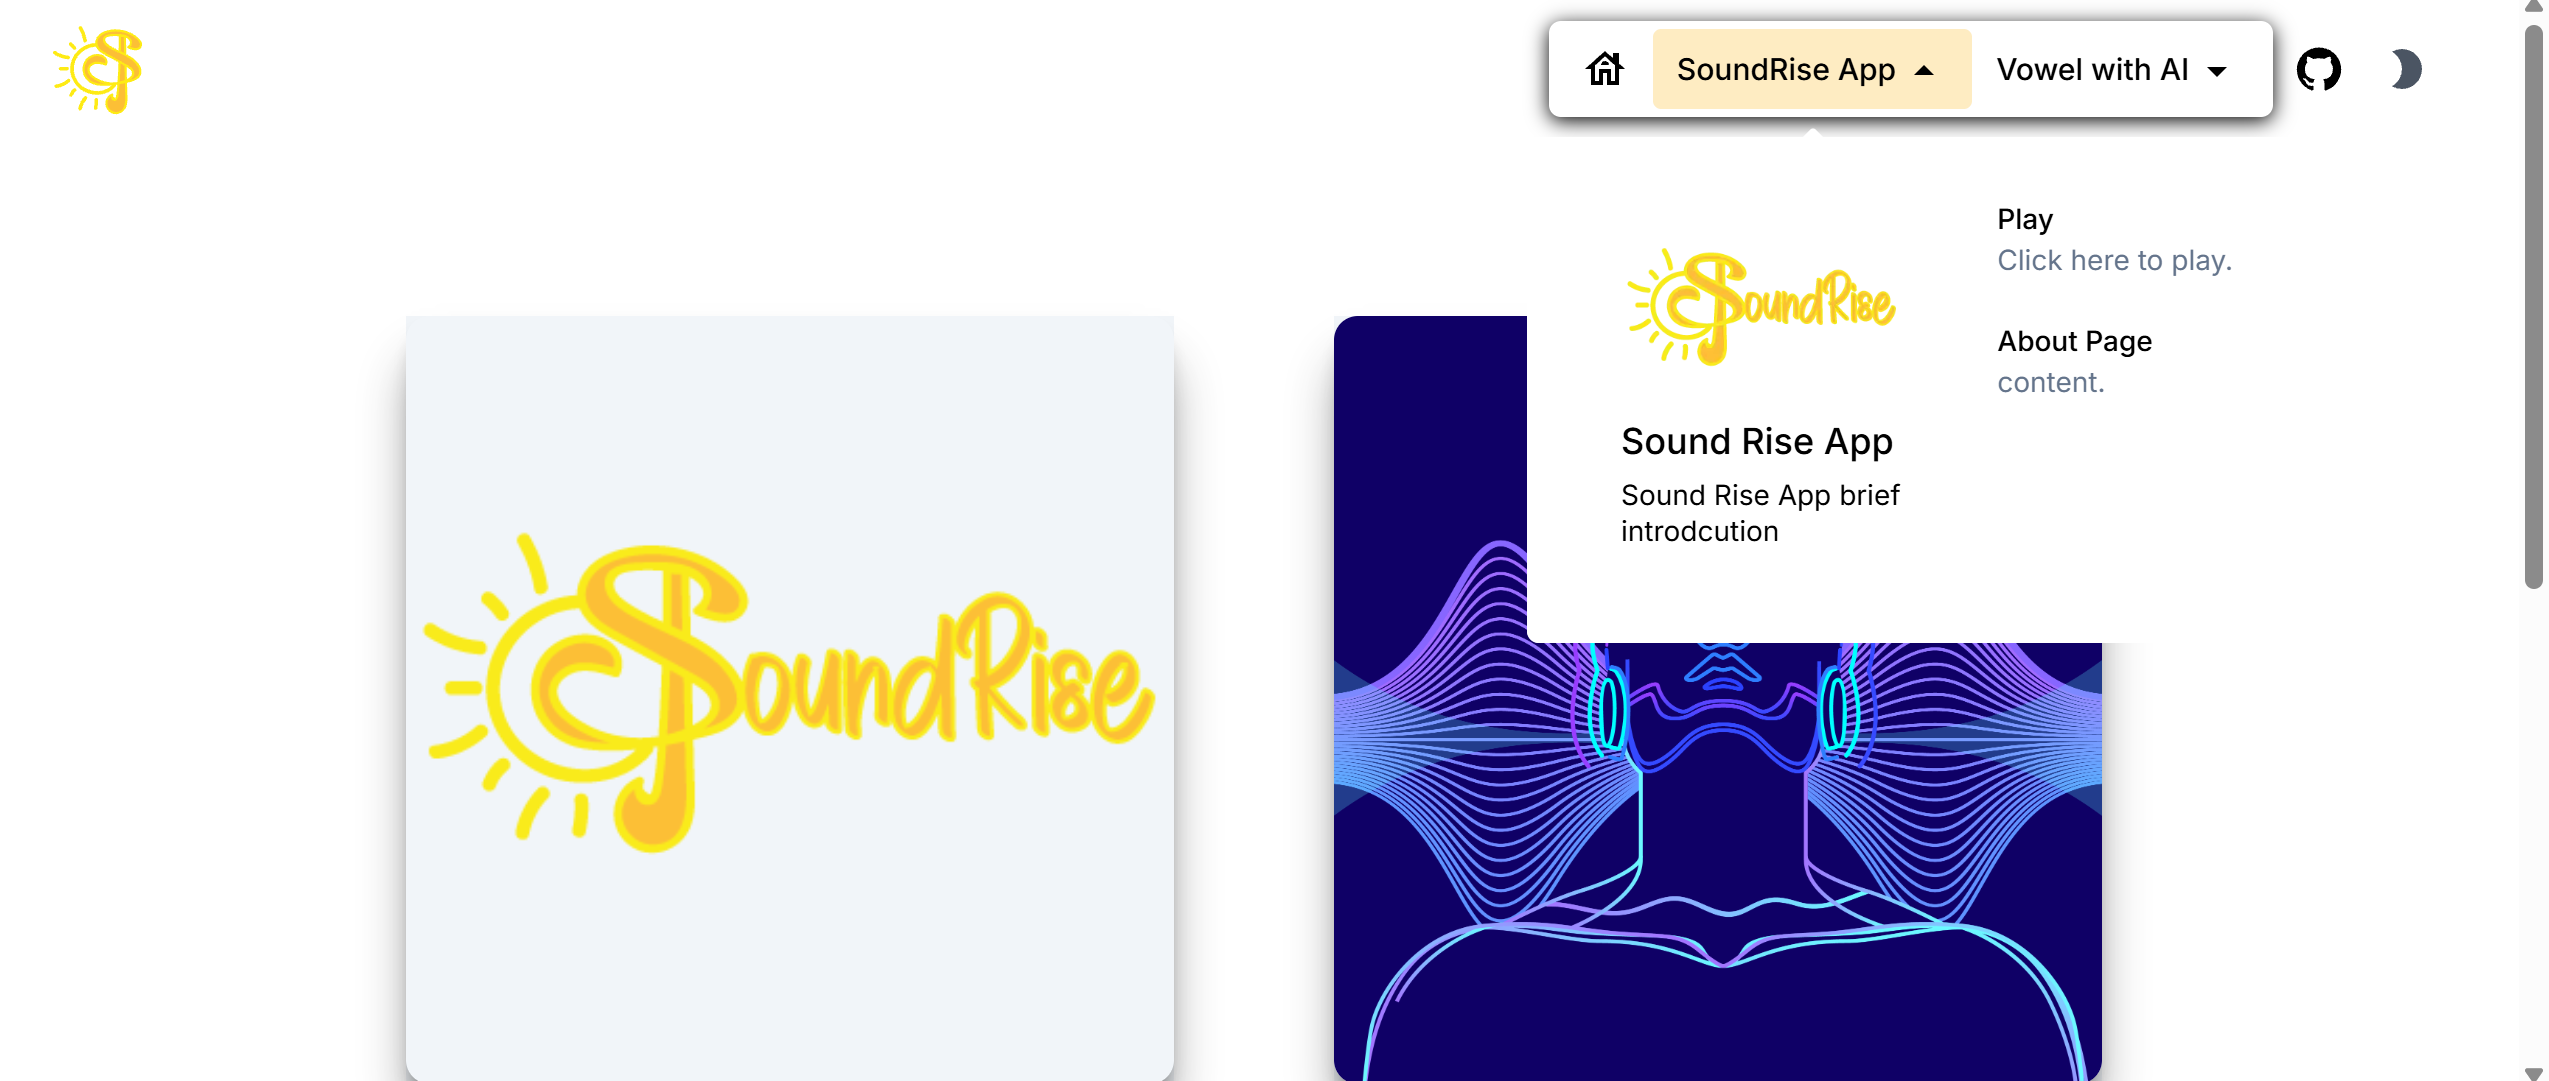
\includegraphics[width=0.8\textwidth]{res/images/webapp/homepage-1.png}
    \caption{SoundRise Homepage Interface}
    \label{fig:homepage}
\end{figure}

\paragraph{}
The application implements a comprehensive dark mode feature (Figure \ref{fig:dark_mode}) to accommodate different user preferences and environmental conditions. This feature not only enhances visual comfort but also reduces eye strain during extended practice sessions, particularly important for users who may require longer periods of practice.

\begin{figure}[htbp]
    \centering
    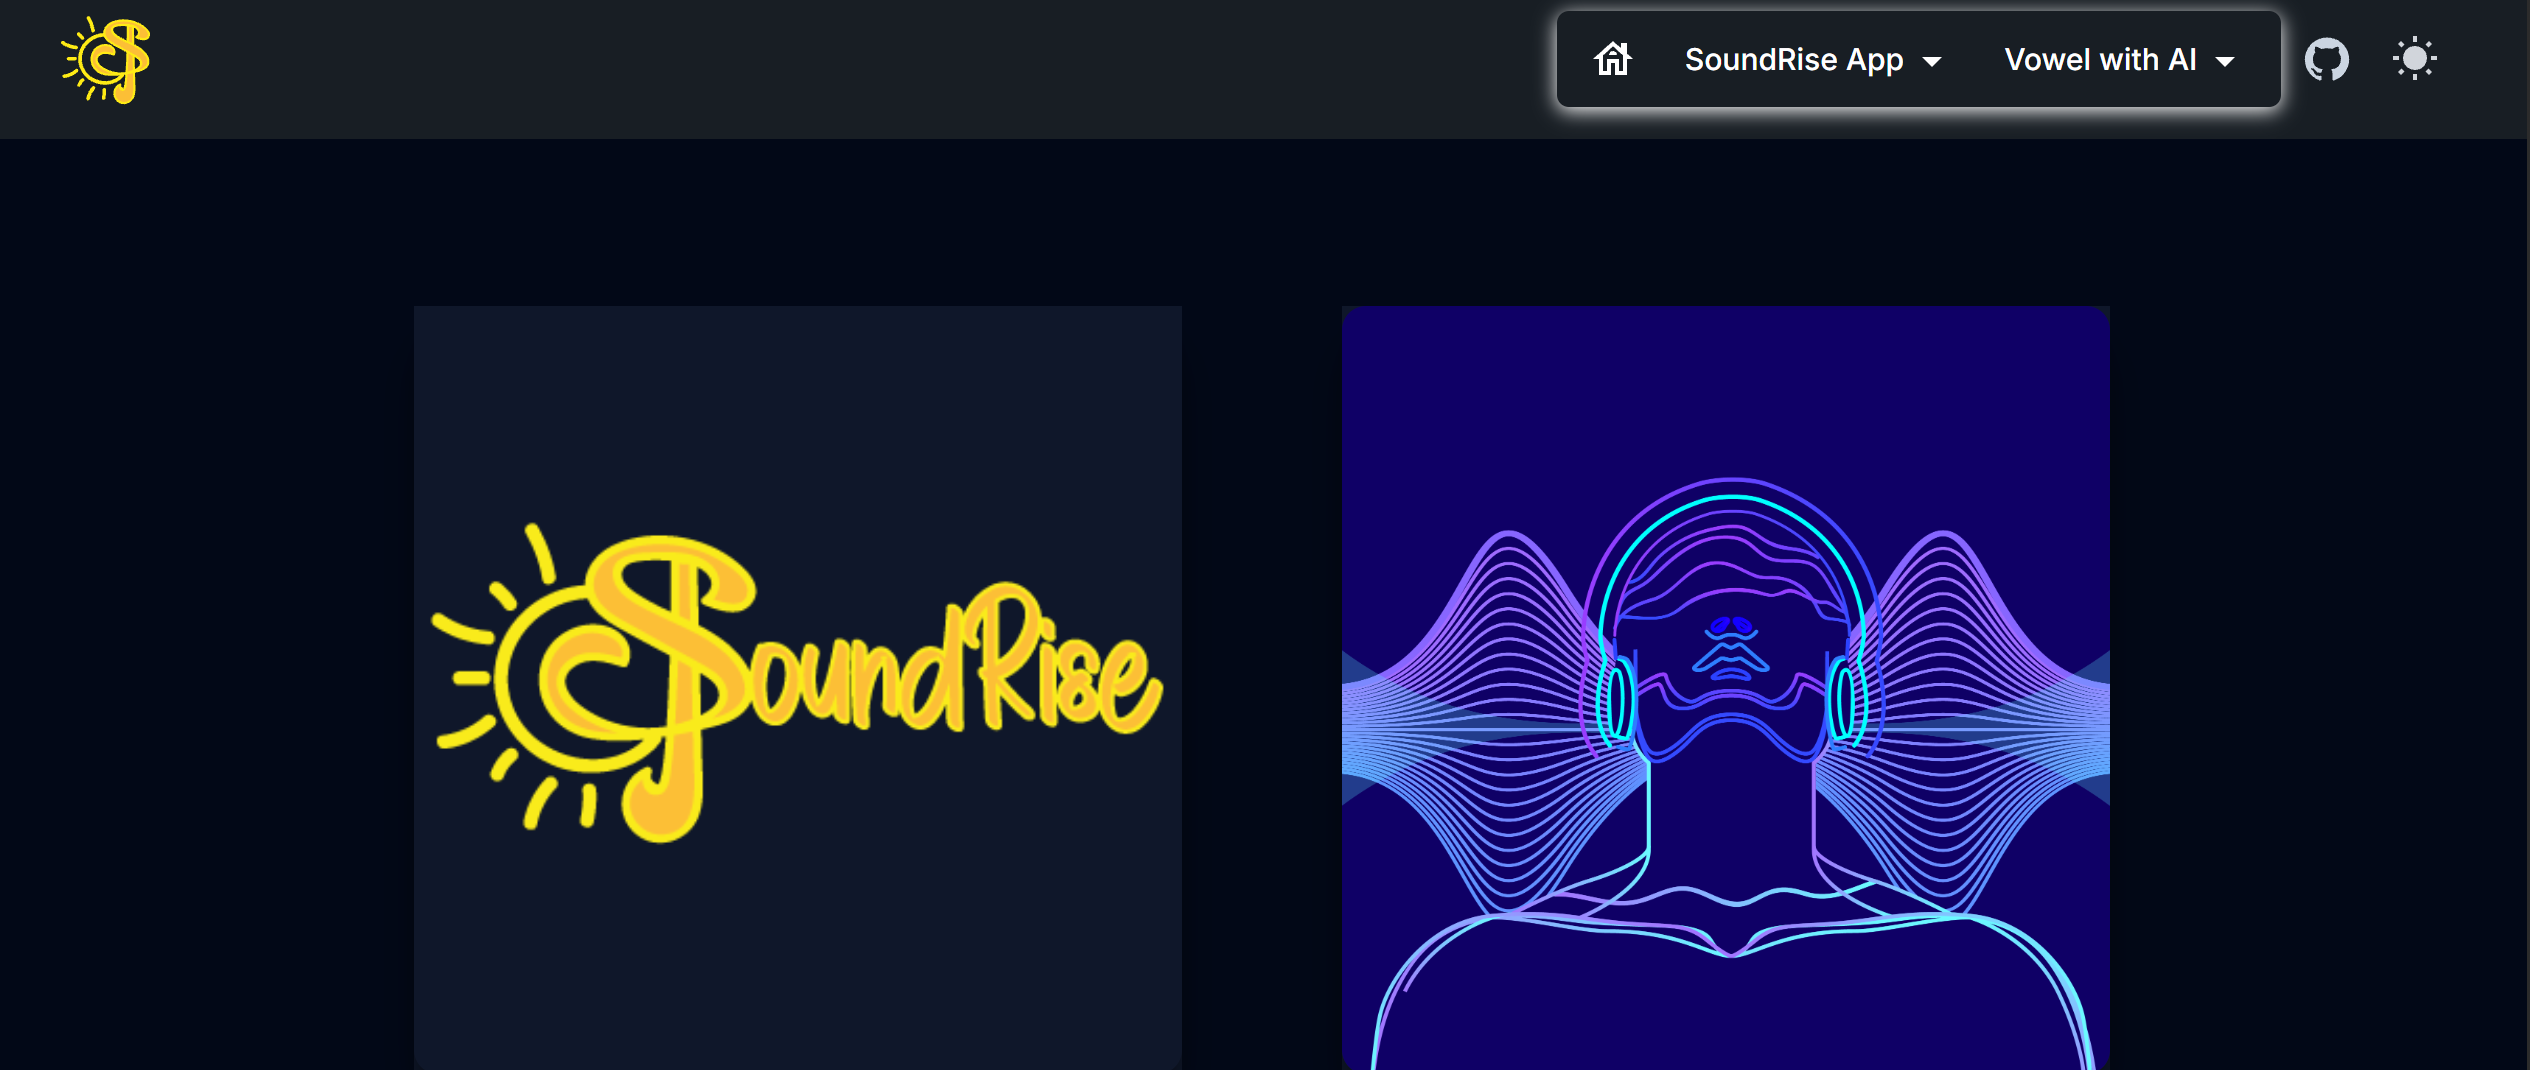
\includegraphics[width=0.8\textwidth]{res/images/webapp/homepage-darkMode.png}
    \caption{Dark Mode Interface}
    \label{fig:dark_mode}
\end{figure}

\paragraph{}
The header section (Figure \ref{fig:header}) provides clear navigation and system status information, including documentation access and user settings. This consistent header design maintains user orientation throughout the application while providing quick access to essential features and help resources.

\begin{figure}[htbp]
    \centering
    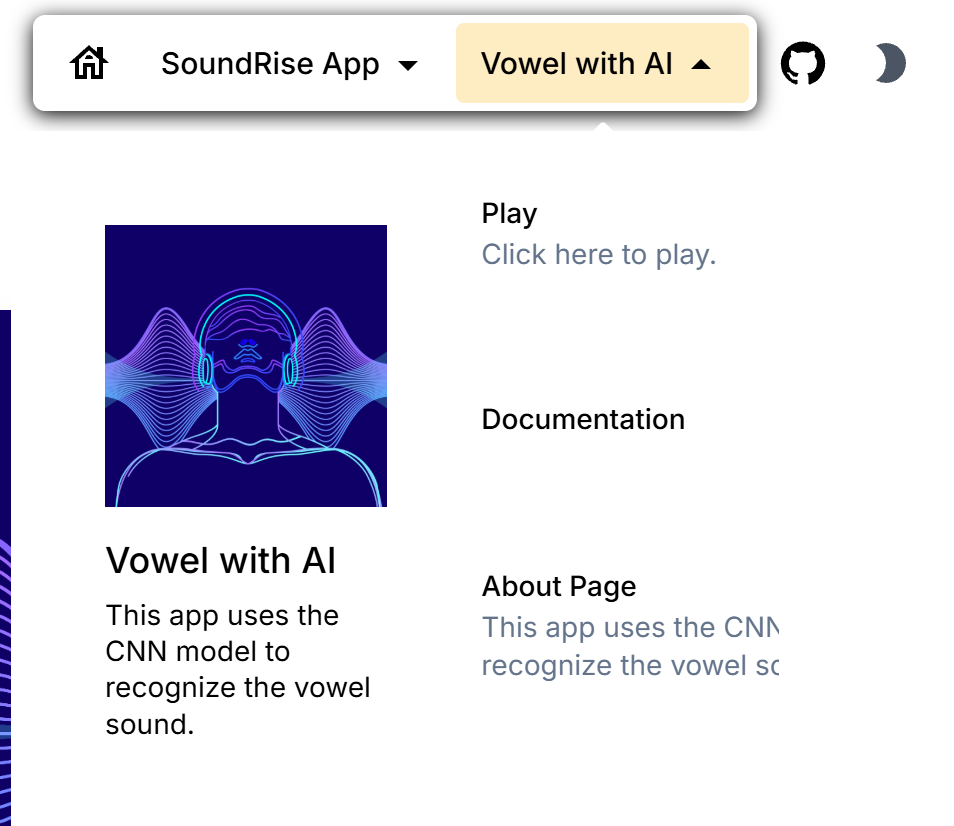
\includegraphics[width=0.8\textwidth]{res/images/webapp/homepage-header.png}
    \caption{Application Header with Navigation Elements}
    \label{fig:header}
\end{figure}

\section{Training Interface Implementation}
\label{sec:training-interface}

\paragraph{}
The training interface (Figure \ref{fig:interface_training}) represents the core functionality of the application, providing real-time feedback during vowel pronunciation practice. The interface combines audio recording controls with visual feedback mechanisms, creating an engaging and informative practice environment.

\begin{figure}[htbp]
    \centering
    
\includegraphics[width=0.8\textwidth]{res/images/webapp/interface.png}
    \caption{Main Training Interface}
    \label{fig:interface_training}
\end{figure}

\paragraph{}
The SoundRise information panel (Figure \ref{fig:info}) displays detailed metrics including pitch and intensity measurements, along with a comprehensive note grid for musical reference. This integration of musical elements helps users understand the relationship between pitch, intensity, and correct vowel pronunciation, providing multiple perspectives for improvement.

\begin{figure}[htbp]
    \centering
    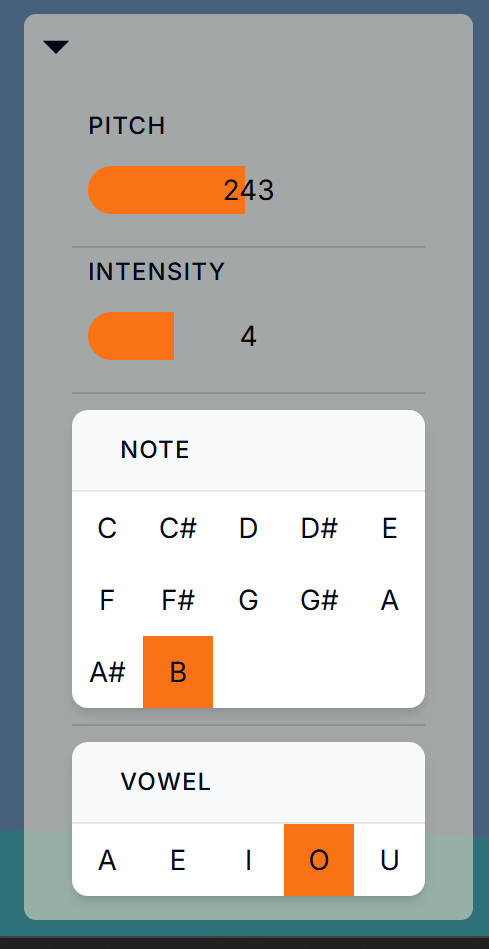
\includegraphics[width=0.4\textwidth]{res/images/webapp/soundRise-info.png}
    \caption{SoundRise Information Panel}
    \label{fig:info}
\end{figure}

\paragraph{}
The interactive feedback system (Figure \ref{fig:feedback}) uses emoticon-based visual cues to provide immediate, intuitive feedback on pronunciation accuracy. This gamification element helps maintain user engagement while providing clear indicators of performance, particularly beneficial for younger users or those new to speech therapy.

\begin{figure}[htbp]
    \centering
    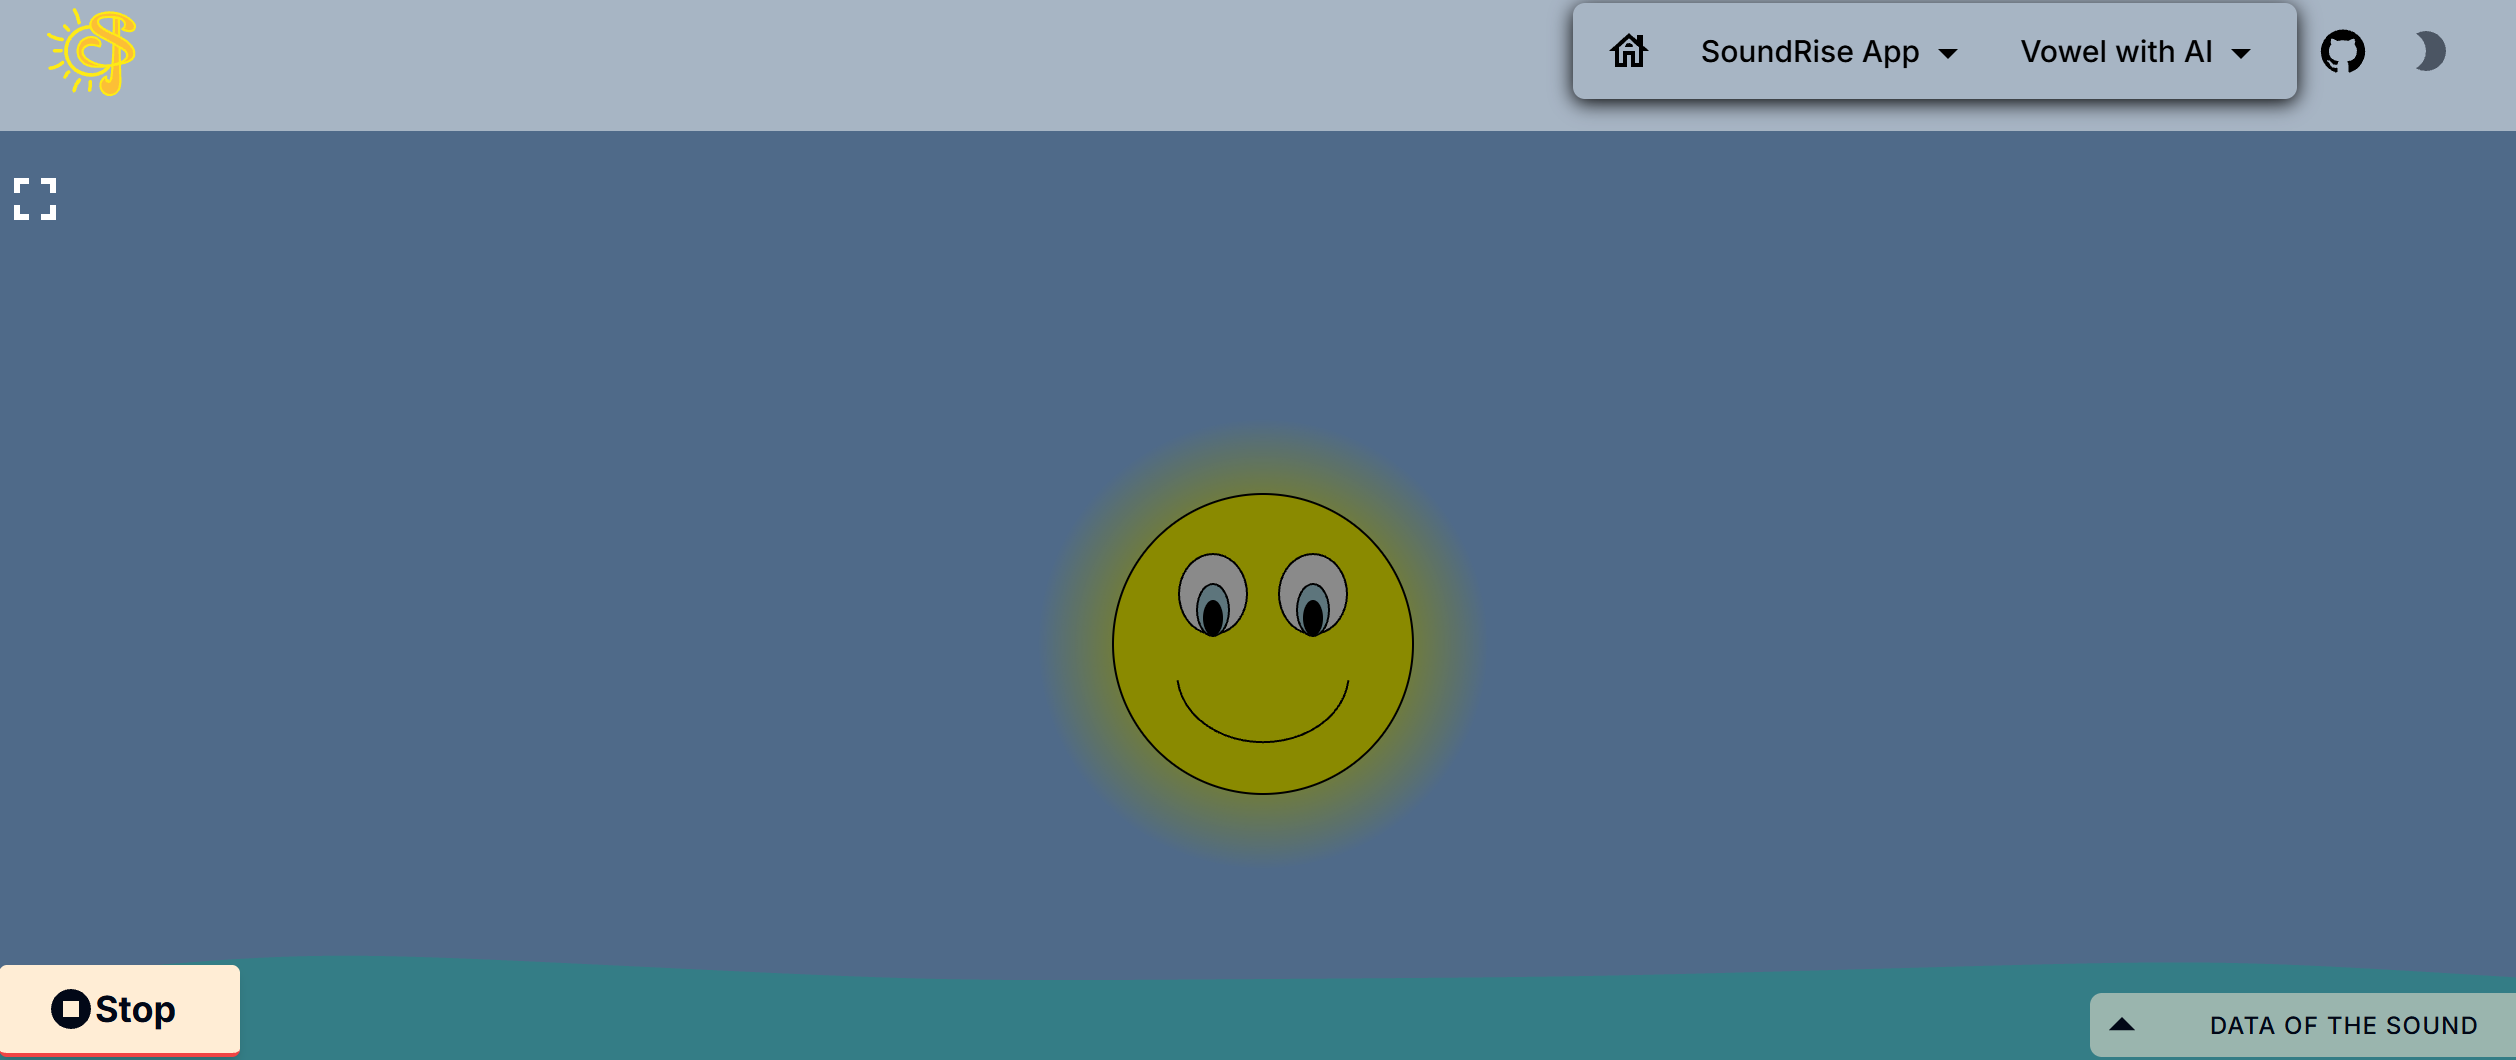
\includegraphics[width=0.4\textwidth]{res/images/webapp/soundRise-1.png}
    \caption{Interactive Feedback Display}
    \label{fig:feedback}
\end{figure}

\section{Results Visualization}
\label{sec:results-visualization}

\paragraph{}
The results interface (Figure \ref{fig:test_result}) provides comprehensive analysis of each pronunciation attempt. The visualization includes spectral analysis, confidence scores, and detailed feedback on pronunciation accuracy, presented in an accessible format that helps users understand their performance.

\begin{figure}[htbp]
    \centering
    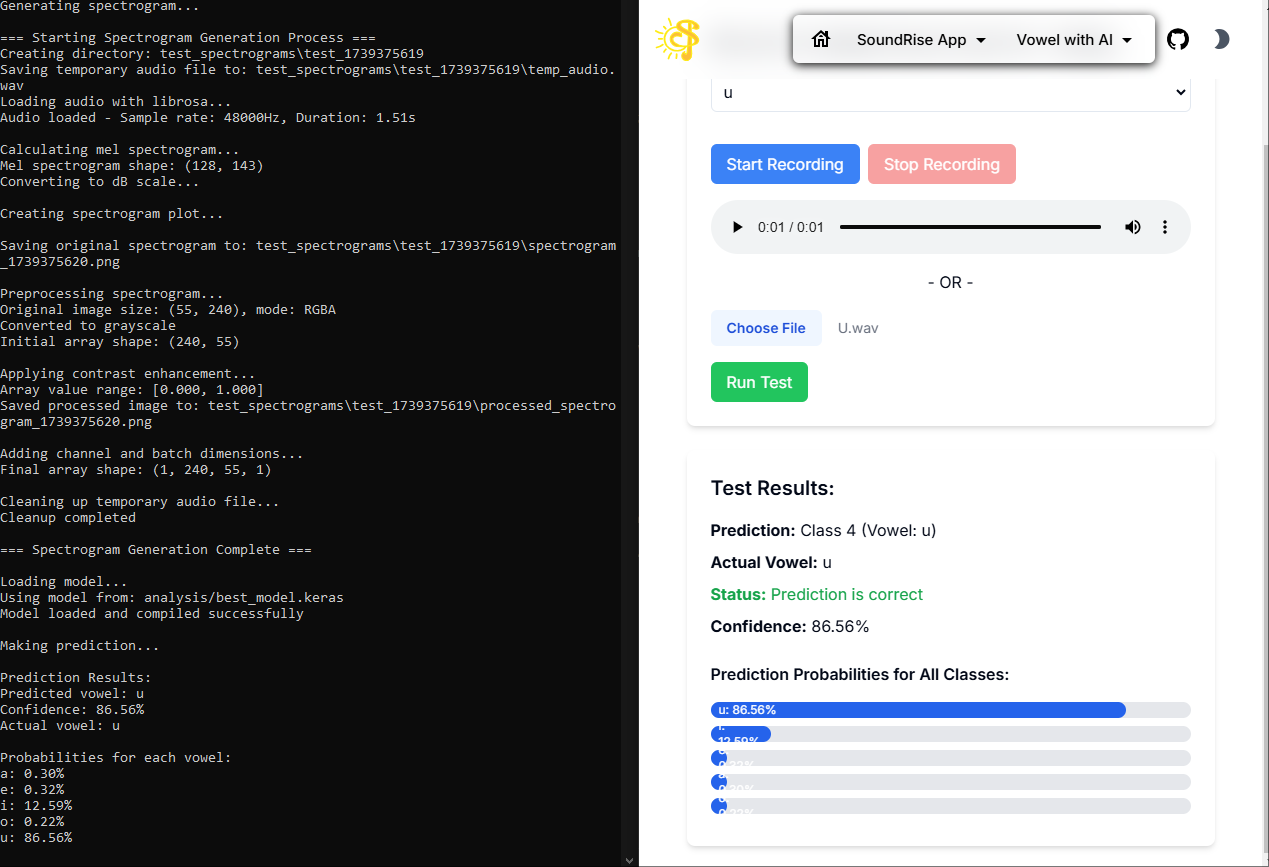
\includegraphics[width=0.8\textwidth]{res/images/webapp/testResult.png}
    \caption{Test Results Interface}
    \label{fig:test_result}
\end{figure}

\paragraph{}
The system implements a sophisticated visualization pipeline that processes real-time audio data and presents it in multiple formats. Users can view their pronunciation attempts through waveform displays, spectrogram visualizations, and numerical metrics, providing multiple perspectives on their performance.

\paragraph{}
Performance tracking features maintain detailed records of practice sessions and achievement metrics. The interface presents this data through intuitive visualizations that help users and therapists monitor progress over time, identify areas for improvement, and adjust practice strategies accordingly.


    %!TEX root = ../main.tex

\chapter{Conclusions and Future Works}
\label{chp:conclusions}

\section{Summary of Achievements}
\label{sec:achievements}

\paragraph{}
This thesis has presented a comprehensive study on vowel recognition using Convolutional Neural Networks, specifically designed for Italian language speech therapy applications. The key achievements of this research include:

\paragraph{}
First, we have successfully developed and implemented a CNN-based vowel recognition system that achieves exceptional accuracy across all Italian vowels. The model demonstrates remarkable stability and robustness, with consistent performance across different batch sizes and training configurations. Our system achieved an overall validation accuracy of 98.77%, with perfect recognition (100%) for vowels 'A' and 'U', and near-perfect accuracy exceeding 99% for other vowels. The performance remained stable across various batch sizes, demonstrating the model's robustness.

\paragraph{}
Second, the system has been successfully integrated into a web-based application platform, making it accessible and user-friendly for speech therapy applications. The implementation features real-time audio processing capabilities, interactive visual feedback mechanisms, cross-platform compatibility, and an efficient client-server architecture that ensures smooth operation across different devices and browsers.

\section{Research Implications}
\label{sec:implications}

\paragraph{}
The findings of this research have several important implications:

\paragraph{}
For Speech Therapy: The high accuracy and real-time processing capabilities of our system make it a valuable tool for speech therapists working with individuals with hearing impairments. The system's ability to provide immediate feedback can enhance the effectiveness of therapy sessions and enable more engaging practice opportunities.

\paragraph{}
For Technical Development: Our implementation demonstrates the viability of using deep learning approaches for specialized speech recognition tasks. The successful integration of CNNs with spectral analysis provides a framework for similar applications in speech processing.

\paragraph{}
For Educational Applications: The web-based nature of our solution makes it accessible for remote learning and self-practice, potentially expanding the reach of speech therapy resources.

\section{Future Research Directions}
\label{sec:future-directions}

\paragraph{}
While the current implementation shows promising results, several areas warrant further investigation:

\subsection{Data Collection and Diversity}
\label{subsec:data-future}

\paragraph{}
A primary focus for future work should be expanding and diversifying the dataset through collaboration with speech therapy clinics and schools. We propose organizing recording sessions with children of different age groups who are currently receiving speech therapy. This would provide invaluable real-world data that captures the natural variations in pronunciation patterns among children with speech disorders. The recordings should be conducted in controlled environments but with varying conditions to ensure robustness.

\paragraph{}
Additionally, we recommend collecting audio samples from different demographic groups, including various age ranges, gender distributions, and regional accents within Italy. This diversity in the training data would enhance the model's ability to generalize across different speaker characteristics and speech patterns.

\subsection{Technical Enhancements}
\label{subsec:technical-future}

\paragraph{}
Future technical developments should focus on expanding the model's capabilities to recognize more complex phonetic elements and implementing real-time noise reduction techniques. The system could be optimized for mobile devices to increase accessibility, and adaptive learning capabilities could be developed to personalize the experience for each user based on their progress and specific challenges.

\subsection{Clinical Applications}
\label{subsec:clinical-future}

\paragraph{}
Further research in clinical applications should include conducting extensive clinical trials with speech therapy patients, developing personalized training programs based on individual progress, and integrating comprehensive progress tracking and reporting features. The system could also be expanded to support other languages while maintaining its effectiveness for Italian vowel recognition.

\section{Final Remarks}
\label{sec:final-remarks}

\paragraph{}
This research has demonstrated the potential of applying modern deep learning techniques to speech therapy applications. The achieved results suggest that our approach could significantly contribute to the field of speech therapy, particularly for individuals with hearing impairments. While there are areas for improvement and expansion, the current implementation provides a solid foundation for future developments in this important domain.

\paragraph{}
The combination of high accuracy, real-time processing, and web-based accessibility makes this system a promising tool for both clinical and educational applications. As technology continues to advance, the integration of such AI-powered tools in speech therapy is likely to become increasingly important in supporting individuals with speech and hearing challenges.


    
    % Bibliography, appendix, acknowledges, etc...
    \backmatter
\end{document}